% Options for packages loaded elsewhere
%DIF LATEXDIFF DIFFERENCE FILE
%DIF DEL OriginallySubmittedVersion.tex   Wed Jan 10 16:23:40 2024
%DIF ADD RevisedVersion.tex               Wed Jan 17 11:16:06 2024
\PassOptionsToPackage{unicode}{hyperref}
\PassOptionsToPackage{hyphens}{url}
%
\documentclass[
]{article}
\usepackage{amsmath,amssymb}
\usepackage{iftex}
\ifPDFTeX
  \usepackage[T1]{fontenc}
  \usepackage[utf8]{inputenc}
  \usepackage{textcomp} % provide euro and other symbols
\else % if luatex or xetex
  \usepackage{unicode-math} % this also loads fontspec
  \defaultfontfeatures{Scale=MatchLowercase}
  \defaultfontfeatures[\rmfamily]{Ligatures=TeX,Scale=1}
\fi
\usepackage{lmodern}
\ifPDFTeX\else
  % xetex/luatex font selection
\fi
% Use upquote if available, for straight quotes in verbatim environments
\IfFileExists{upquote.sty}{\usepackage{upquote}}{}
\IfFileExists{microtype.sty}{% use microtype if available
  \usepackage[]{microtype}
  \UseMicrotypeSet[protrusion]{basicmath} % disable protrusion for tt fonts
}{}
\makeatletter
\@ifundefined{KOMAClassName}{% if non-KOMA class
  \IfFileExists{parskip.sty}{%
    \usepackage{parskip}
  }{% else
    \setlength{\parindent}{0pt}
    \setlength{\parskip}{6pt plus 2pt minus 1pt}}
}{% if KOMA class
  \KOMAoptions{parskip=half}}
\makeatother
\usepackage{xcolor}
\usepackage[vmargin=1in,hmargin=1in]{geometry}
\usepackage{longtable,booktabs,array}
\usepackage{calc} % for calculating minipage widths
% Correct order of tables after \paragraph or \subparagraph
\usepackage{etoolbox}
\makeatletter
\patchcmd\longtable{\par}{\if@noskipsec\mbox{}\fi\par}{}{}
\makeatother
% Allow footnotes in longtable head/foot
\IfFileExists{footnotehyper.sty}{\usepackage{footnotehyper}}{\usepackage{footnote}}
\makesavenoteenv{longtable}
\usepackage{graphicx}
\makeatletter
\def\maxwidth{\ifdim\Gin@nat@width>\linewidth\linewidth\else\Gin@nat@width\fi}
\def\maxheight{\ifdim\Gin@nat@height>\textheight\textheight\else\Gin@nat@height\fi}
\makeatother
% Scale images if necessary, so that they will not overflow the page
% margins by default, and it is still possible to overwrite the defaults
% using explicit options in \includegraphics[width, height, ...]{}
\setkeys{Gin}{width=\maxwidth,height=\maxheight,keepaspectratio}
% Set default figure placement to htbp
\makeatletter
\def\fps@figure{htbp}
\makeatother
\setlength{\emergencystretch}{3em} % prevent overfull lines
\providecommand{\tightlist}{%
  \setlength{\itemsep}{0pt}\setlength{\parskip}{0pt}}
\setcounter{secnumdepth}{-\maxdimen} % remove section numbering
% definitions for citeproc citations
\NewDocumentCommand\citeproctext{}{}
\NewDocumentCommand\citeproc{mm}{%
  \begingroup\def\citeproctext{#2}\cite{#1}\endgroup}
\makeatletter
 % allow citations to break across lines
 \let\@cite@ofmt\@firstofone
 % avoid brackets around text for \cite:
 \def\@biblabel#1{}
 \def\@cite#1#2{{#1\if@tempswa , #2\fi}}
\makeatother
\newlength{\cslhangindent}
\setlength{\cslhangindent}{1.5em}
\newlength{\csllabelwidth}
\setlength{\csllabelwidth}{3em}
\newenvironment{CSLReferences}[2] % #1 hanging-indent, #2 entry-spacing
 {\begin{list}{}{%
  \setlength{\itemindent}{0pt}
  \setlength{\leftmargin}{0pt}
  \setlength{\parsep}{0pt}
  % turn on hanging indent if param 1 is 1
  \ifodd #1
   \setlength{\leftmargin}{\cslhangindent}
   \setlength{\itemindent}{-1\cslhangindent}
  \fi
  % set entry spacing
  \setlength{\itemsep}{#2\baselineskip}}}
 {\end{list}}
\usepackage{calc}
\newcommand{\CSLBlock}[1]{\hfill\break\parbox[t]{\linewidth}{\strut\ignorespaces#1\strut}}
\newcommand{\CSLLeftMargin}[1]{\parbox[t]{\csllabelwidth}{\strut#1\strut}}
\newcommand{\CSLRightInline}[1]{\parbox[t]{\linewidth - \csllabelwidth}{\strut#1\strut}}
\newcommand{\CSLIndent}[1]{\hspace{\cslhangindent}#1}
\usepackage{amsmath}
\usepackage{pdflscape,booktabs}
\newcommand{\blandscape}{\begin{landscape}}
\newcommand{\elandscape}{\end{landscape}}
\usepackage[running]{lineno}
\linenumbers
\ifLuaTeX
  \usepackage{selnolig}  % disable illegal ligatures
\fi
\usepackage{bookmark}
\IfFileExists{xurl.sty}{\usepackage{xurl}}{} % add URL line breaks if available
\urlstyle{same}
\hypersetup{
  hidelinks,
  pdfcreator={LaTeX via pandoc}}

\author{}
\date{\vspace{-2.5em}}
%DIF PREAMBLE EXTENSION ADDED BY LATEXDIFF
%DIF UNDERLINE PREAMBLE %DIF PREAMBLE
\RequirePackage[normalem]{ulem} %DIF PREAMBLE
\RequirePackage{color}\definecolor{RED}{rgb}{1,0,0}\definecolor{BLUE}{rgb}{0,0,1} %DIF PREAMBLE
\providecommand{\DIFadd}[1]{{\protect\color{blue}\uwave{#1}}} %DIF PREAMBLE
\providecommand{\DIFdel}[1]{{\protect\color{red}\sout{#1}}}                      %DIF PREAMBLE
%DIF SAFE PREAMBLE %DIF PREAMBLE
\providecommand{\DIFaddbegin}{} %DIF PREAMBLE
\providecommand{\DIFaddend}{} %DIF PREAMBLE
\providecommand{\DIFdelbegin}{} %DIF PREAMBLE
\providecommand{\DIFdelend}{} %DIF PREAMBLE
\providecommand{\DIFmodbegin}{} %DIF PREAMBLE
\providecommand{\DIFmodend}{} %DIF PREAMBLE
%DIF FLOATSAFE PREAMBLE %DIF PREAMBLE
\providecommand{\DIFaddFL}[1]{\DIFadd{#1}} %DIF PREAMBLE
\providecommand{\DIFdelFL}[1]{\DIFdel{#1}} %DIF PREAMBLE
\providecommand{\DIFaddbeginFL}{} %DIF PREAMBLE
\providecommand{\DIFaddendFL}{} %DIF PREAMBLE
\providecommand{\DIFdelbeginFL}{} %DIF PREAMBLE
\providecommand{\DIFdelendFL}{} %DIF PREAMBLE
\newcommand{\DIFscaledelfig}{0.5}
%DIF HIGHLIGHTGRAPHICS PREAMBLE %DIF PREAMBLE
\RequirePackage{letltxmacro} %DIF PREAMBLE
\newsavebox{\DIFdelgraphicsbox} %DIF PREAMBLE
\newlength{\DIFdelgraphicswidth} %DIF PREAMBLE
\newlength{\DIFdelgraphicsheight} %DIF PREAMBLE
% store original definition of \includegraphics %DIF PREAMBLE
\LetLtxMacro{\DIFOincludegraphics}{\includegraphics} %DIF PREAMBLE
\newcommand{\DIFaddincludegraphics}[2][]{{\color{blue}\fbox{\DIFOincludegraphics[#1]{#2}}}} %DIF PREAMBLE
\newcommand{\DIFdelincludegraphics}[2][]{% %DIF PREAMBLE
\sbox{\DIFdelgraphicsbox}{\DIFOincludegraphics[#1]{#2}}% %DIF PREAMBLE
\settoboxwidth{\DIFdelgraphicswidth}{\DIFdelgraphicsbox} %DIF PREAMBLE
\settoboxtotalheight{\DIFdelgraphicsheight}{\DIFdelgraphicsbox} %DIF PREAMBLE
\scalebox{\DIFscaledelfig}{% %DIF PREAMBLE
\parbox[b]{\DIFdelgraphicswidth}{\usebox{\DIFdelgraphicsbox}\\[-\baselineskip] \rule{\DIFdelgraphicswidth}{0em}}\llap{\resizebox{\DIFdelgraphicswidth}{\DIFdelgraphicsheight}{% %DIF PREAMBLE
\setlength{\unitlength}{\DIFdelgraphicswidth}% %DIF PREAMBLE
\begin{picture}(1,1)% %DIF PREAMBLE
\thicklines\linethickness{2pt} %DIF PREAMBLE
{\color[rgb]{1,0,0}\put(0,0){\framebox(1,1){}}}% %DIF PREAMBLE
{\color[rgb]{1,0,0}\put(0,0){\line( 1,1){1}}}% %DIF PREAMBLE
{\color[rgb]{1,0,0}\put(0,1){\line(1,-1){1}}}% %DIF PREAMBLE
\end{picture}% %DIF PREAMBLE
}\hspace*{3pt}}} %DIF PREAMBLE
} %DIF PREAMBLE
\LetLtxMacro{\DIFOaddbegin}{\DIFaddbegin} %DIF PREAMBLE
\LetLtxMacro{\DIFOaddend}{\DIFaddend} %DIF PREAMBLE
\LetLtxMacro{\DIFOdelbegin}{\DIFdelbegin} %DIF PREAMBLE
\LetLtxMacro{\DIFOdelend}{\DIFdelend} %DIF PREAMBLE
\DeclareRobustCommand{\DIFaddbegin}{\DIFOaddbegin \let\includegraphics\DIFaddincludegraphics} %DIF PREAMBLE
\DeclareRobustCommand{\DIFaddend}{\DIFOaddend \let\includegraphics\DIFOincludegraphics} %DIF PREAMBLE
\DeclareRobustCommand{\DIFdelbegin}{\DIFOdelbegin \let\includegraphics\DIFdelincludegraphics} %DIF PREAMBLE
\DeclareRobustCommand{\DIFdelend}{\DIFOaddend \let\includegraphics\DIFOincludegraphics} %DIF PREAMBLE
\LetLtxMacro{\DIFOaddbeginFL}{\DIFaddbeginFL} %DIF PREAMBLE
\LetLtxMacro{\DIFOaddendFL}{\DIFaddendFL} %DIF PREAMBLE
\LetLtxMacro{\DIFOdelbeginFL}{\DIFdelbeginFL} %DIF PREAMBLE
\LetLtxMacro{\DIFOdelendFL}{\DIFdelendFL} %DIF PREAMBLE
\DeclareRobustCommand{\DIFaddbeginFL}{\DIFOaddbeginFL \let\includegraphics\DIFaddincludegraphics} %DIF PREAMBLE
\DeclareRobustCommand{\DIFaddendFL}{\DIFOaddendFL \let\includegraphics\DIFOincludegraphics} %DIF PREAMBLE
\DeclareRobustCommand{\DIFdelbeginFL}{\DIFOdelbeginFL \let\includegraphics\DIFdelincludegraphics} %DIF PREAMBLE
\DeclareRobustCommand{\DIFdelendFL}{\DIFOaddendFL \let\includegraphics\DIFOincludegraphics} %DIF PREAMBLE
%DIF END PREAMBLE EXTENSION ADDED BY LATEXDIFF

\begin{document}

\section{The complex network of trophic interactions in a subAntarctic
oceanic Marine Protected
Area}\label{the-complex-network-of-trophic-interactions-in-a-subantarctic-oceanic-marine-protected-area}

\subsection{Abstract}\label{abstract}

The total area of the world ocean designated under marine protection has
increased recently. Most Marine Protected Areas (MPAs) target
vulnerable, keystone, charismatic and or endemic species. In the
sub-Antarctic, ocean protection is associated to oceanic islands, except
for MPAs Namuncurá - Burdwood Bank I and II (MPA N-BB,
\textasciitilde53º--55ºS and \textasciitilde56º--62ºW), which are
associated to a submarine plateau and its southern adjacent deep slope,
respectively. Here, we present the first analysis of the network of
predator-prey interactions for the MPA N-BB. We applied a \DIFaddbegin \DIFadd{topological
}\DIFaddend network approach to characterise the complexity and structure of the
food web, and identify the species' role in such a framework. The MPA
N-BB food web consisted of 1788 interactions and 379 species, with a
connectance of 0.01. Almost half of the consumers were omnivores \DIFaddbegin \DIFadd{or
feeding at more than one trophic level }\DIFaddend (0.48), and the network displayed
a small-world pattern \DIFdelbegin \DIFdel{. These suggest }\DIFdelend \DIFaddbegin \DIFadd{(short path length, high clustering of
compartments). This network pattern suggests }\DIFaddend that the ecosystem might be
vulnerable to perturbations targeting highly connected species, although
\DIFdelbegin \DIFdel{other }\DIFdelend \DIFaddbegin \DIFadd{some }\DIFaddend properties might provide resilience and resistance, resulting in a
rearranged structure that preserves its original functions. Several
species arose as important in terms of different aspects of trophic
structure and functioning, and response to perturbations. Generalist
species, mainly fishes, play a crucial role in the ecosystem's
benthopelagic coupling and should be considered as relevant energy
transfers for the ecosystem. We argue that the diversity of species,
including both the benthic and pelagic habitats, is responsible for
securing the connectivity within the food web against perturbations,
therefore contributing to the structure and stability of the ecosystem.

Keywords: Food Web, Complexity, Structure, Burdwood Bank, Southwest
Atlantic

\subsection{1. Introduction}\label{introduction}

\DIFdelbegin \DIFdel{The evidence of
benefits provided by }\DIFdelend \DIFaddbegin \DIFadd{In recent years, there has been an unprecedented rise in the number of
}\DIFaddend Marine Protected Areas (MPAs) \DIFdelbegin \DIFdel{as
well as the urgent }\DIFdelend \DIFaddbegin \DIFadd{worldwide, driven by both the compelling
evidence of their benefits and the pressing }\DIFaddend need for ocean protection
\DIFdelbegin \DIFdel{have driven an
unprecedented increase in the number of MPAs worldwide in recent years
}\DIFdelend (Roberts et al., 2017; Sala et al., 2018). Globally, the total area of
the world ocean designated under marine protection adds up to
approximately 29,600,000 km\textsuperscript{2}, distributed across
nearly 18,444 MPAs and covering 8.16\% of the ocean's surface (IUCN and
UNEP-WCMC, 2023), and therefore approaching the 10\% goal of the
Convention of Biological Diversity (Secretariat of the convention on
biological diversity, 2004). \DIFdelbegin \DIFdel{Despite this progress , recent reports have
shown that actual }\DIFdelend \DIFaddbegin \DIFadd{Although some progress has been made, it
has become apparent that the level of }\DIFaddend protection has been \DIFdelbegin \DIFdel{overestimated because it includes
areas that are not yet effectively protected (only declared) as }\DIFdelend \DIFaddbegin \DIFadd{inflated due
to the inclusion of regions that have only been declared as protected,
as }\DIFaddend well as areas \DIFdelbegin \DIFdel{that allow significant extractive activities }\DIFdelend \DIFaddbegin \DIFadd{where significant extractive operations are allowed
}\DIFaddend (Sala et al., 2018).

In the sub-Antarctic region, the level of ocean protection is mainly
associated to oceanic islands, such as the South Georgias and South
Sandwich, Bouvet, Prince Edward, and Macquarie islands (IUCN and
UNEP-WCMC, 2023). Interestingly, the case of the \DIFaddbegin \DIFadd{Argentine }\DIFaddend MPAs
Namuncurá - Burdwood Bank I and II (MPA N-BB, \textasciitilde53º--55ºS
\textasciitilde56º--62ºW), which is the focus of this work, is unique
since these MPAs are associated to a submarine plateau and its southern
adjacent deep slope region, respectively (Falabella, 2017; Schejter et
al., 2020). In addition, such MPAs are part of a network of protected
areas in the sub-Antarctic area (jointly with MPA Yaganes) that aims to
protect this southern region in order to contribute to global ocean
health.

Many of these MPAs focus on the presence of particularly vulnerable,
keystone, or charismatic species, large numbers (or proportions) of
endemic species, and/or high biodiversity across taxonomic levels (Hogg
et al., 2016). Indeed, the MPA N-BB was created to protect a potentially
sensitive and biodiverse benthic habitat that was only barely known
(Falabella, 2017; Schejter et al., 2016). The benthic community is
featured by high biomass of vulnerable and fragile species (mainly
Porifera, Bryozoa and Cnidaria) that\DIFaddbegin \DIFadd{, }\DIFaddend considered with their environment\DIFaddbegin \DIFadd{,
}\DIFaddend meet the characteristics of vulnerable marine ecosystems (Schejter and
Albano, 2021), here defined as sites that present densities of Indicator
Taxa of \textgreater{} 10 kg per 1200 m\textsuperscript{2} (Commission
for the Conservation of Antarctic Marine Living Resources (CCAMLR),
2009). Also, the benthic realm provides habitat to several small-sized
species (López-Gappa et al., 2018; Martin Sirito, 2019; Schejter and
Bremec, 2019), and has an important role in the life history of fishes
as a food source, refuge and nursery area (Covatti Ale et al., 2022;
Delpiani et al., 2020; Fischer et al., 2022; Florencia et al., 2023;
García Alonso et al., 2018; Matusevich, 2022; Troccoli et al., 2020;
Vazquez et al., 2018). The maintenance of this singular community is
related to local and regional oceanographic processes, including the
circulation of the rich Malvinas \DIFdelbegin \DIFdel{(Falkland) }\DIFdelend current in the area (Guerrero et al.,
1999; Piola and Gordon, 1989) and the upwelling and mixing phenomena
(Matano et al., 2019). The input of nutrients from the Malvinas \DIFdelbegin \DIFdel{(Falkland) }\DIFdelend current
also supports a diverse plankton community (Guinder et al., 2020). \DIFaddbegin \DIFadd{Given
the cooling trend of this current in a warming regional context
(i.e.~adjacent waters of the Patagonian shelf and Southwest Atlantic
Ocean) (Franco et al., 2022), the MPA N-BB might play an essential role
as a refuge maintaining not only the biodiversity but also the
fisheries' populations of the region (Franco et al., 2020b).
}\DIFaddend 

\DIFaddbegin \DIFadd{Identifying the main species involved in the maintenance of ecosystem
services and health as well as for management and conservation is
essential. In this regard, Bergagna et al. (2020) have identified the
principal ecosystem services that are provided by species inhabiting the
MPA N-BB; for instance, nursery and feeding areas for commercially
important fishes (e.g.~Patagonian grenadier }\emph{\DIFadd{Macruronus
magellanicus}}\DIFadd{, Patagonian toothfish }\emph{\DIFadd{Dissostichus eleginoides}}\DIFadd{),
water purification by filter feeders (e.g.~sponges), among others. These
species are part of a complex system in terms of biodiversity. There is
robust knowledge on the complexity considering the richness of the
benthic and plankton communities in the MPA N-BB ecosystem
(Administración de Parques Nacionales, 2022; Guinder et al., 2020;
Schejter et al., 2020, 2016). }\DIFaddend Overall, 811 benthic and plankton species
have been identified \DIFdelbegin \DIFdel{for }\DIFdelend \DIFaddbegin \DIFadd{in }\DIFaddend the MPA N-BB ecosystem, where 349 were reported
for the first time in the area in recent years (Administración de
Parques Nacionales, 2022). \DIFdelbegin \DIFdel{Identifying the main species involved in the maintenance of ecosystem
services and health as well as for management and conservation is
essential. }\DIFdelend Recently, the structure of the southwestern
South Atlantic Ocean has been \DIFdelbegin \DIFdel{proposed }\DIFdelend \DIFaddbegin \DIFadd{hypothesised }\DIFaddend to be under a `wasp-waist'
control, meaning that the structure and dynamics of the ecosystem are
regulated primarily by mid-trophic level species (e.g., fishes,
crustaceans) (Padovani et al., 2012; Riccialdelli et al., 2020; Saporiti
et al., 2015). In particular, the ecosystem of the MPA N-BB shows a more
pronounced `wasp-waist' structure, meaning a shorter \DIFaddbegin \DIFadd{average }\DIFaddend food chain
and a greater trophic overlap and redundancy, than other sub-Antarctic
areas \DIFdelbegin \DIFdel{, }\DIFdelend such as the continental shelf off Tierra del Fuego. \DIFaddbegin \DIFadd{It is the high
abundance of few prey species at this mid-trophic level of the food web
which imposes a certain feeding dependence to high-trophic level
predators, shortens food-web length and increases the trophic overlap
and redundancy of the overall food web. }\DIFaddend The Fuegian sprat \emph{Sprattus
fuegensis} and longtail southern cod \DIFdelbegin \emph{\DIFdel{Patagonotothen ramsayi}} %DIFAUXCMD
\DIFdelend \DIFaddbegin \DIFadd{Patagonotothen ramsayi }\DIFaddend are
considered the most plausible `wasp-waist' species\DIFdelbegin \DIFdel{(Riccialdelli }\DIFdelend \DIFaddbegin \DIFadd{, since they are
species with high regional abundances (Arkhipkin and Laptikhovsky, 2013;
Madirolas }\DIFaddend et al., \DIFdelbegin \DIFdel{2020).
}%DIFDELCMD < 

%DIFDELCMD < %%%
\DIFdel{High-latitude marine ecosystems, such as the MPA N-BB, are complex
systems in terms of biodiversity and ecological interactions (Cordone }\DIFdelend \DIFaddbegin \DIFadd{2000), occupy mid-trophic levels (Riccialdelli }\DIFaddend et al.,
2020\DIFdelbegin \DIFdel{; Day et al., 2013; Kortsch et al., 2019; Trathan }\DIFdelend \DIFaddbegin \DIFadd{, 2010), many predators feed on them (Riccialdelli }\DIFaddend et al., \DIFdelbegin \DIFdel{2021). Although there is a robust knowledge about the complexity
considering the richness of the benthic and plankton communities in the
MPA N-BB ecosystem (Administración de Parques Nacionales, 2022; Guinder
et al., 2020; Schejter }\DIFdelend \DIFaddbegin \DIFadd{2020),
and the population dynamics of these species appear to depend on the
environment (e.g.~climatic variations) (Diez }\DIFaddend et al., \DIFdelbegin \DIFdel{2020, 2016), a better }\DIFdelend \DIFaddbegin \DIFadd{2018). These recent
efforts have increased our understanding of the biological communities
and their complexity, but an }\DIFaddend understanding of species interactions'
complexity and structure is \DIFdelbegin \DIFdel{needed. }\DIFdelend \DIFaddbegin \DIFadd{lacking. Such understanding will provide a
more complete picture of the ecosystem, generate a baseline to
comprehend climate change effects for the region (Franco et al., 2020b)
and serve as an input to decision makers on conservation actions
(Administración de Parques Nacionales, 2022).
}

\DIFaddend This aspect can be tackled by analysing one of the most frequent
relationships between species: the predator-prey interaction (Bascompte,
2009). The sum of \DIFdelbegin \DIFdel{predator-prey or trophic interactions of }\DIFdelend \DIFaddbegin \DIFadd{these interactions in }\DIFaddend a particular region is referred
to as a food web, representing the roadmap for matter and energy flow in
an ecosystem. In recent years, \DIFaddbegin \DIFadd{topological }\DIFaddend network approaches have been
successfully applied to study complex high-latitude marine ecosystems,
improving our knowledge on structure, functioning, and response to
environmental/anthropogenic changes (Cordone et al., 2018; Funes et al.,
2022; Kortsch et al., 2015; Marina et al., 2023). Among anthropogenic
threats, it is worth mentioning that contaminants like mercury and
microplastics have been recently reported as important threats to the
MPA N-BB region (Cossi et al., 2021; Di Mauro et al., 2022; Fioramonti
et al., 2022); also fishing vessels are allowed to operate in the
western section of the MPA N-BB (i.e.~Marine National Reserve category),
altering the stocks of commercially important fish species
(Administración de Parques Nacionales, 2022; Martínez et al., 2021).
Moreover, there is a potential hazard related to the effects of offshore
activities (exploration and \DIFdelbegin \DIFdel{explotation}\DIFdelend \DIFaddbegin \DIFadd{exploitation of gas and oil}\DIFaddend ) to the west of
the MPA N-BB (Administración de Parques Nacionales, 2022).

In \DIFdelbegin \DIFdel{the present }\DIFdelend \DIFaddbegin \DIFadd{this }\DIFaddend work, we present the first detailed analysis of the network of
predator-prey interactions, hereafter food web, for the MPA N-BB
ecosystem. For this, we applied a \DIFaddbegin \DIFadd{topological }\DIFaddend network approach to a
highly resolved food web. The objective was twofold: characterise the
food web in terms of complexity and structure, and identify the species'
role in the network. \DIFaddbegin \DIFadd{For the former, we considered all species and
interactions in the food web, and calculated the number of species (S),
number of interactions (L), link density (L/S), connectance (L/S\^{}2),
proportion of omnivorous, and assessed the small-world pattern. For the
latter objective, we considered interactions and species related to a
particular species and analyse the following properties: betweenness,
closeness, trophic similarity, topological role and trophic level.
}\DIFaddend 

\subsection{2. Methodology}\label{methodology}

\subsubsection{2.1. Study area}\label{study-area}

The MPAs Namuncurá - Burdwood Bank I and II, created by \DIFaddbegin \DIFadd{Argentine
}\DIFaddend National Laws 26.875 in 2013 and 27.490 in 2017, comprise a shallow
submarine plateau called Burdwood Bank (BB) and a deep slope \DIFaddbegin \DIFadd{to the
south }\DIFaddend that reaches 4000 m in depth, N-BB I and N-BB II, respectively
(Administración de Parques Nacionales, 2022; Tombesi et al., 2020)
(Figure 1). They are located 150 km east of Isla de los Estados and 200
km south of Malvinas/Falkland Islands. The MPA N-BB I comprises nearly
28,900 km\textsuperscript{2} circumscribed by the 200 m isobath, between
\textasciitilde54º--55ºS and \textasciitilde56º--62ºW, with a slight
slope \DIFdelbegin \DIFdel{extended }\DIFdelend \DIFaddbegin \DIFadd{extending }\DIFaddend nearly 370 km east--west. \DIFdelbegin \DIFdel{Physical features in the BBare fairly }\DIFdelend \DIFaddbegin \DIFadd{The physical characteristics
of the BB's deep waters are relatively }\DIFaddend stable, with \DIFdelbegin \DIFdel{salinity
averaging }\DIFdelend \DIFaddbegin \DIFadd{a consistent
salinity of }\DIFaddend 34 \DIFdelbegin \DIFdel{all year round and temperature ranging between 4 }\DIFdelend \DIFaddbegin \DIFadd{psu throughout the year }\DIFaddend and \DIFaddbegin \DIFadd{a temperature range of 4 to
}\DIFaddend 8ºC (Acha et al., 2004; Guerrero et al., 1999; Piola and Falabella,
2009). The BB is \DIFdelbegin \DIFdel{surrounded by steep flanks }\DIFdelend \DIFaddbegin \DIFadd{enclosed by high, steep slopes that plunge to depths }\DIFaddend of
up to 4000 m\DIFdelbegin \DIFdel{depth through which
strong currents circulate }\DIFdelend \DIFaddbegin \DIFadd{, where powerful currents flow }\DIFaddend (Matano et al., 2019; Piola
and Gordon, 1989; Reta, 2014). The N-BB II includes such a deep slope,
protecting about 32,000 km\textsuperscript{2} (\textasciitilde55º-56ºS,
\textasciitilde58º-62ºW). Intense upwelling and mixing \DIFdelbegin \DIFdel{occur in
relation
}\DIFdelend \DIFaddbegin \DIFadd{take place in
connection }\DIFaddend with the slope, \DIFdelbegin \DIFdel{entraining deep}\DIFdelend \DIFaddbegin \DIFadd{bringing deep, }\DIFaddend nutrient-rich waters into the
photic layer (Matano et al., 2019; Piola and Falabella, 2009) and
resulting in a \DIFdelbegin \DIFdel{fairly homogeneous }\DIFdelend \DIFaddbegin \DIFadd{relatively uniform }\DIFaddend water column both \DIFdelbegin \DIFdel{spatially and
temporally
}\DIFdelend \DIFaddbegin \DIFadd{horizontally and
vertically, both in space and time }\DIFaddend (Glorioso and Flather, 1995; Guerrero
et al., 1999; Matano et al., 2019).

Given the evidence collected during several research cruises about the
oceanographic and ecological processes connecting MPAs N-BB I and II
(references in Administración de Parques Nacionales, 2022), a joint
management plan was recently proposed (Administración de Parques
Nacionales, 2022). This is why, the study area of the present work
includes both MPAs.

\subsubsection{2.2. Network construction}\label{network-construction}

In order to build the network of predator-prey interactions, we \DIFdelbegin \DIFdel{reviewed
}\DIFdelend \DIFaddbegin \DIFadd{started
by searching trophic information for the species reported by Schejter et
al. (2016) and Falabella (2017). Subsequently, we performed a literature
search using the name of the species in question and the keywords
`diet', `prey', `predator', `feeding ecology' and `trophic ecology' in
Google Scholar and Scopus. This process identified }\DIFaddend more than 170
references \DIFdelbegin \DIFdel{considering }\DIFdelend \DIFaddbegin \DIFadd{including peer-reviewed }\DIFaddend published articles, Ph.D.~theses,
public databases, and reports belonging to 16 research cruises conducted
in the MPAs N-BB I and II during 2014-2019. \DIFdelbegin \DIFdel{It is noteworthy that the
sampling effort was greater in the MPA N-BB I. Furthermore, we took into
account personal communications from }\DIFdelend \DIFaddbegin \DIFadd{We considered that one
reference showing evidence of a predator-prey relationship was enough to
add that interaction to the network. Finally, we consulted with }\DIFaddend experts
belonging to the working group of the study area
(\url{https://www.pampazul.gob.ar/tag/banco-burdwood/}) \DIFaddbegin \DIFadd{that filtered
the list of trophic interactions and discarded those unlikely to occur
in the MPAs N-BB I and II}\DIFaddend . The diversity of the authors' expertise
contributing to the present study was a key factor in enhancing the
quality of the network, and inherently improved the network
representation. A list of the references used to build the network is
presented in Supplementary Material (Table S1).

Due to a lack of trophic data resolution for some species inhabiting the
study area, we followed the concept of trophic species, here defined as
follows: taxa collapsed into a single node in the network. In most
cases, we followed this concept when specific data on species, in the
taxonomic sense, were not available. In some cases, we collapsed species
when taxa shared the same set of predators and prey (trophic similarity,
Martinez (1991)), one of the aggregation methods that better preserve
food web functional properties (Gauzens et al., 2013). In addition, for
endemic species (e.g.~bryozoan \emph{Burdwoodipora paguricola}) and
other species with no trophic studies so far, we inferred their feeding
interactions applying a conservative approach that assumes that the set
of prey and predators are at some point preserved in time. In those
cases we gathered information from upper taxonomic levels (i.e.~Genus,
Family, Order, Class, Phylum) as a good proxy variable (Morales-Castilla
et al., 2015; Pomeranz et al., 2019). Details about this can be found in
Supplementary Material (Table S2). Furthermore, we considered non-living
food sources, such as detritus and necromass, as prey species in the
food web context.

With the gathered trophic data, we constructed a matrix of pairwise
interactions; a value of 1 or 0 was assigned to each element a\_ij of
the matrix depending on whether the \DIFdelbegin \DIFdel{j-species }\DIFdelend \DIFaddbegin \DIFadd{predator j }\DIFaddend preyed or not on the \DIFdelbegin \DIFdel{i-species}\DIFdelend \DIFaddbegin \DIFadd{prey
i}\DIFaddend . Then we transformed such a matrix into an \DIFdelbegin \DIFdel{oriented }\DIFdelend \DIFaddbegin \DIFadd{directed }\DIFaddend graph with L
trophic interactions between S nodes or species \DIFdelbegin \DIFdel{. The orientation or
}\DIFdelend \DIFaddbegin \DIFadd{(Supplementary Material,
Figure S1). The }\DIFaddend direction of the \DIFaddbegin \DIFadd{interaction within the }\DIFaddend graph follows
the flow of energy and matter in the network, from prey to predator.

\subsubsection{2.3. Network analysis}\label{network-analysis}

We analysed the MPA N-BB network of trophic interactions, or food web,
at two levels: A) network, considering species and interactions of the
whole network; and B) species, considering interactions and species
related to a particular species (Table 1).

The network-level analysis aims to characterise the food web in terms of
complexity and structure. For this, we calculated several network
properties commonly used to describe empirical food webs (Pascual and
Dunne, 2005): (1) number of species \DIFdelbegin \DIFdel{S}\DIFdelend \DIFaddbegin \DIFadd{\(S\)}\DIFaddend ; (2) number of interactions or
links \DIFdelbegin \DIFdel{L}\DIFdelend \DIFaddbegin \DIFadd{\(L\)}\DIFaddend ; (3) link density \DIFdelbegin \DIFdel{L/S}\DIFdelend \DIFaddbegin \DIFadd{\(L/S\)}\DIFaddend ; (4) connectance \DIFdelbegin \DIFdel{L/S\^{}2}\DIFdelend \DIFaddbegin \DIFadd{\(L/S^2\)}\DIFaddend ; (5)
omnivory \DIFdelbegin \DIFdel{Omn}\DIFdelend \DIFaddbegin \DIFadd{\(Omn\)}\DIFaddend ; and (6) small-world pattern. In order to explore the
small-world phenomenon, we analysed the characteristic path length
(\DIFdelbegin \DIFdel{CPL}\DIFdelend \DIFaddbegin \DIFadd{\(CPL\)}\DIFaddend ) and the clustering coefficient (\DIFdelbegin \DIFdel{CC}\DIFdelend \DIFaddbegin \DIFadd{\(CC\)}\DIFaddend ). The \DIFdelbegin \DIFdel{CPL }\DIFdelend \DIFaddbegin \DIFadd{\(CPL\) }\DIFaddend is the
average shortest path length between all pairs of nodes (Watts and
Strogatz, 1998). Here, \DIFdelbegin \DIFdel{CPL }\DIFdelend \DIFaddbegin \DIFadd{\(CPL\) }\DIFaddend was calculated as the average number of
nodes in the shortest path \(CPL_{Min} (i,j)\) between all pairs of
nodes \(S(i,j)\) in a network averaged over \(S(S-1)/2\) nodes:

\DIFdelbegin \[
\DIFdel{CPL = \frac{2}{S(S-1)} \sum_{i = 1}^{S} \sum_{i = 1}^{S} }{\DIFdel{CPL_{Min}(i,j)}}
\DIFdel{}\]%DIFAUXCMD
\DIFdelend \DIFaddbegin \begin{align}
\DIFadd{CPL = \frac{2}{S(S-1)} \sum_{i = 1}^{S} \sum_{ij = 1}^{S} }{\DIFadd{CPL_{Min}(i,j)}}
\DIFadd{}\end{align}\DIFaddend 
\DIFdelbegin \DIFdel{The CC }\DIFdelend \DIFaddbegin 

\DIFadd{The \(CC\) }\DIFaddend quantifies the local interconnectedness of the network and it
is defined as the fraction of the number of existing links between
neighbours of node \(i\) among all possible links between these
neighbours. In this study, the \DIFdelbegin \DIFdel{CC }\DIFdelend \DIFaddbegin \DIFadd{\(CC\) }\DIFaddend was determined as the average of
the individual clustering coefficients \(CC_i\) of all the nodes in the
network. Individual \(CC_i\) were determined as follows:

\DIFdelbegin \[
\DIFdel{CC_i = \frac{2E_i}{K_i(K_i-1)}
}\]%DIFAUXCMD
\DIFdelend \DIFaddbegin \begin{align}
\DIFadd{CC_i = \frac{2E_i}{K_i(K_i-1)}
}\end{align}\DIFaddend 
\DIFaddbegin 

\DIFaddend where \(E_i\) is the effective number of interactions between \(K_i\)
nearest-neighbour nodes of node \(i\) and the maximal possible number of
such interactions (Newman, 2003). To test whether the food web presented
the small-world pattern, we compared the empirical values of \DIFdelbegin \DIFdel{CPL and
CC
}\DIFdelend \DIFaddbegin \DIFadd{\(CPL\) and
\(CC\) }\DIFaddend with those resulting from 1000 randomly generated networks with
the same size (\DIFdelbegin \DIFdel{S}\DIFdelend \DIFaddbegin \DIFadd{\(S\)}\DIFaddend ) and number of interactions (\DIFdelbegin \DIFdel{L)}\DIFdelend \DIFaddbegin \DIFadd{\(L\)). Random webs
were created using the Erdös-Rényi model, where links are added to the
complete set of nodes (\(S\)) and chosen uniformly randomly from the set
of all possible links (Erdös and Rényi}\DIFaddend , \DIFdelbegin \DIFdel{following the
method proposed
by }\DIFdelend \DIFaddbegin \DIFadd{1959). The rigurosity of our
method lies in the use of confidence intervals (CI 99\%) for the
empirical-random comparison of the \(CPL\) and \(CC\) properties. If the
empirical value is positioned within or to the left (= lower than) the
CI 99\% of the random CPL, and to the right (= higher than) the CI 99\%
of the CC, then the food web is considered to present the SW topology
(}\DIFaddend Marina et al.\DIFdelbegin \DIFdel{(}\DIFdelend \DIFaddbegin \DIFadd{, }\DIFaddend 2018b).

Also, we estimated the (7) degree distributions for the food web, prey
and predators, and each functional group (e.g., Amphipoda, Ascidiacea,
Bivalvia, fish, marine mammals, seabirds, among others). The prey and
predator distributions indicate the frequency of prey among predators,
and viceversa; the functional group's degree shows the distribution of
interactions within groups.

The species-level analysis aims to describe the species' role in the
food web. For this, we considered the following properties: betweenness
\DIFdelbegin \DIFdel{Btw, closeness Cl}\DIFdelend \DIFaddbegin \DIFadd{\(Btw\), closeness \(Cl\)}\DIFaddend , trophic similarity \DIFdelbegin \DIFdel{TS}\DIFdelend \DIFaddbegin \DIFadd{\(TS\)}\DIFaddend , topological role
\DIFdelbegin \DIFdel{TR}\DIFdelend \DIFaddbegin \DIFadd{\(TR\)}\DIFaddend , and trophic level \DIFdelbegin \DIFdel{TL }\DIFdelend \DIFaddbegin \DIFadd{\(TL\) }\DIFaddend (Table 1). Topological roles refer to
the fact that food webs tend to naturally organize in non-random,
modular patterns, where modules are defined as a group of species that
interact more frequently among themselves than with species that are not
members of the module (Guimerà and Nunes Amaral, 2005). \DIFaddbegin \DIFadd{This means that
groups of prey and predators interact more strongly with each other,
than with species belonging to other groups. Modularity measures how
strongly these subgroups of species, called modules, interact with each
other compared to species from other modules. }\DIFaddend Species can play different
roles in this respect, according to the pattern of interactions within
their own module and/or across modules. We computed the topological role
for each species, classified as module hub, species with a relatively
high number of interactions, but most within its own module; module
specialist, species with relatively few interactions and most within its
own module; module connector, species with relatively few interactions
mainly between modules; and network connector, species with high
connectivity between and within modules (Guimerà and Nunes Amaral,
2005). \DIFaddbegin \DIFadd{Refer to the Supplementary Material for the equations used to
calculate the species-level properties.
}\DIFaddend 

We also studied the relationship between species \DIFdelbegin \DIFdel{TL }\DIFdelend \DIFaddbegin \DIFadd{\(TL\) }\DIFaddend and the other
species properties by \DIFdelbegin \DIFdel{performing linear regression }\DIFdelend \DIFaddbegin \DIFadd{fitting }\DIFaddend analyses. Thus, we considered the \DIFdelbegin \DIFdel{TL }\DIFdelend \DIFaddbegin \DIFadd{\(TL\)
}\DIFaddend as the dependent variable and the given property (i.e.~betweenness,
closeness, trophic similarity) as the independent variable\DIFdelbegin \DIFdel{and obtained the coefficients (slope and intercept) for the linear model. Models were fitted using the least squares approach.}\DIFdelend \DIFaddbegin \DIFadd{. Fitting was
done locally, meaning that for the fit at point }\emph{\DIFadd{x}}\DIFadd{, the fit is
made using points in a neighborhood of }\emph{\DIFadd{x}}\DIFadd{, weighted by their
distance from }\emph{\DIFadd{x}} \DIFadd{(Cleveland et al., 1992). }\DIFaddend We also explored the
topological role categories with the species \DIFdelbegin \DIFdel{TL}\DIFdelend \DIFaddbegin \DIFadd{\(TL\)}\DIFaddend . These species-level
properties provide an appropriate description of species' role in
empirical complex food webs (Cirtwill et al., 2018).

All network analyses and graphs were performed in R version \DIFdelbegin \DIFdel{4.2.2
(}\textbf{\DIFdel{RCoreTeam2022?}}%DIFAUXCMD
\DIFdelend \DIFaddbegin \DIFadd{4.3.1 (Team,
2023}\DIFaddend ), mainly using `igraph' (Csardi and Nepusz, 2006) and `multiweb'
(Saravia, 2022) packages. \DIFaddbegin \DIFadd{Fitting between species \(TL\) and the other
species properties was performed using }\emph{\DIFadd{loess}} \DIFadd{function from
`stats' package (Team, 2023). }\DIFaddend The source code and data are available at
\url{https://github.com/TomasMarina/Banco-Burdwood}.

\subsection{3. Results}\label{results}

\subsubsection{3.1. Network-level
properties}\label{network-level-properties}

In terms of complexity, the MPA \DIFdelbegin \DIFdel{Namuncurá - Burdwood Bank }\DIFdelend \DIFaddbegin \DIFadd{N-BB }\DIFaddend food web consisted of 1788
predator-prey interactions and 379 species, where 93\% of them were
defined at the species taxonomical level (Figure 2, Table S2). The food
web presented a link density (e.g., the average number of interactions
per species) of 4.72, and a connectance of 0.01. Almost half of the
consumers were omnivores (0.48), feeding on sources at different trophic
levels. The food web displayed a small-world pattern, meaning that the
path length was lower and the clustering coefficient higher than the
random networks (Table 2).

The degree distribution of the food web showed an asymmetric frequency
in the number of interactions, where most of the species had a
relatively low number of interactions and few species concentrated most
of them (Figure 3A). The distribution of prey among predators showed
that most consumers fed on a low number of prey whereas few had multiple
prey (Figure 3B). The top-five predators in number of prey were:
yellowfin notothen \emph{Patagonotothen guntheri} (Notothenioid fish, 50
prey), rock cod \emph{Patagonotothen ramsayi} (Notothenioid fish, 49
prey), broad nose skate \emph{Bathyraja brachyurops} (Chondrichthyan, 33
prey), Patagonian toothfish \emph{Dissostichus eleginoides}
(Notothenioid fish, 30 prey), and graytail skate \emph{Bathyraja
griseocauda} (Chondrichthyan, 28 prey). Following the same distribution
pattern, few prey presented multiple predators (Figure 3C). The top-five
prey (or food sources) in number of predators were: Detritus
(Non-living, 153 predators), the three categories of Diatoms considered
(benthic, centric and pennate, 72.5 predators on average), and species
of the genus \emph{Euphausia} (Zooplankton, 46 predators). Finally,
\DIFdelbegin \DIFdel{taking into account the interactions within each functional group }\DIFdelend \DIFaddbegin \DIFadd{aggregating the interactions by functional group (Figure 3D)}\DIFaddend , most
interactions were concentrated in a few species\DIFdelbegin \DIFdel{(Figure 3D)}\DIFdelend . The most evident
species were: \emph{Doryteuthis gahi} (Cephalopoda), \emph{Grimothea
(=Munida) gregaria} (Decapoda), \emph{Patagonotothen ramsayi},
\emph{Patagonotothen guntheri} and \emph{Dissostichus eleginoides}
(bentho-pelagic fish), \emph{Sprattus fuegensis} and
\emph{Micromesistius australis} (pelagic fish), and species of
\emph{Euphausia} and \emph{Themisto gaudichaudii} (Zooplankton).
Overall, there is an evident asymmetry in the distribution of
interactions among species at different levels \DIFaddbegin \DIFadd{(i.e.~considering the
entire food web, gathered by prey, predator and functional group) }\DIFaddend in the
MPA N-BB food web. \DIFdelbegin %DIFDELCMD < 

%DIFDELCMD < %%%
\DIFdelend A list of the distribution of interactions per
species is presented in Supplementary Material (Table S3).

\subsubsection{3.2. Species-level
properties}\label{species-level-properties}

We found different relationships between the species trophic level (TL)
and the rest of the analysed species-level properties (Figure 4A-D). The
most evident \DIFdelbegin \DIFdel{significant }\DIFdelend relationship was with trophic similarity, \DIFaddbegin \DIFadd{which described
an exponential-like decline; }\DIFaddend i.e.~the higher the species' TL, the lower
the trophic similarity or the higher the uniqueness in terms of trophic
role (Figure \DIFdelbegin \DIFdel{4C}\DIFdelend \DIFaddbegin \DIFadd{4A}\DIFaddend ). Here it is noteworthy to highlight those high-trophic
level species (TL \textgreater{} 3.1) with low values of trophic
similarity: \emph{Bathyraja macloviana} and \emph{Squalus acanthias}
(Chondrichthyans), \emph{Diplopteraster clarki} and \emph{Pteraster} sp.
(echinoderms), \emph{Daption capense} and \emph{Eudyptes chrysocome}
(seabirds), Ziphiidae and \emph{Lagenorhynchus cruciger} (marine
mammals) (Table S3).

We also found a \DIFdelbegin \DIFdel{significant }\DIFdelend \DIFaddbegin \DIFadd{general }\DIFaddend negative relationship between TL and closeness,
\DIFdelbegin \DIFdel{however less evident, meaning that low-TL species are
relatively }\DIFdelend \DIFaddbegin \DIFadd{meaning that species with relatively low-TLs are }\DIFaddend closer to any other
species in the food web (Figure 4B). \DIFaddbegin \DIFadd{Specifically, species in the range
2 - 3 showed a hump-shaped distribution, while for TL \textgreater{} 3
closeness decreased consistently. }\DIFaddend Detritus, species of genera
\emph{Calanus} and \emph{Euphausia}, and Foraminifera, all with TL
\textless{} 3, registered the highest closeness values (Table S3).

\DIFdelbegin \DIFdel{Notably, }\DIFdelend \DIFaddbegin \DIFadd{Regarding betweenness, as expected }\DIFaddend species of mid-TLs (3-4.2) showed the
highest values\DIFdelbegin \DIFdel{of
betweenness}\DIFdelend , meaning that those species participated in the highest
number of shortest paths between species (Figure \DIFdelbegin \DIFdel{4A}\DIFdelend \DIFaddbegin \DIFadd{4C}\DIFaddend ). The following are
the species with the highest values (descending order):
\emph{Patagonotothen ramsayi}, \emph{Salilota australis},
\emph{Dissostichus eleginoides} (fishes), \emph{Doryteuthis gahi}
(Cephalopoda), and \emph{Patagonotothen guntheri} (Notothenioid fish)
(Table S3). \DIFaddbegin \DIFadd{Here we should note that species with highest TLs
(\textgreater{} 4.2, top predators) show values equal to zero since no
``betweenness'' role is possible for them.
}\DIFaddend 

Considering the topological role, `module specialist' species were the
most frequent and presented a wide TL range (1 - 4.78), as well as
`module hub' species (TL = 1 - 3.92); `module connector' was constrained
to mid-TLs (2 - 3.86); and `network connector', was represented by only
one trophic species: detritus (Figure 4D, see Figure S2 for species'
topological roles in a food web graph framework). Here it is important
to highlight the two latter topological roles because they are
responsible for linking modules and maintaining the connectivity of the
food web: 42 species (1 network connector + 41 module connectors) from
19 different functional groups with a TL range = 1 - 3.86. The 41
species with a module connector role represented these functional
groups: Amphipoda, Bivalvia, Brachiopoda, Bryozoa, Hydrozoa (as
`Cnidaria\_benthic'), Copepoda, Cumacea, Decapoda, Echinodermata, fish
(bentho-pelagic and demersal Osteichthyes, and Chondrychthyes),
Foraminifera, Polychaeta, Porifera, Pycnogonida (as `Benthos\_Misc') and
zooplankton (see Supplementary Material Table S3 for the identity of the
species). \DIFdelbegin %DIFDELCMD < 

%DIFDELCMD < %%%
\DIFdelend An exhaustive list of the species-level properties is
presented in Supplementary Material (Table S3).

\subsection{4. Discussion}\label{discussion}

\subsubsection{4.1. The food web of the MPA Namuncurá - Burdwood Bank
ecosystem}\label{the-food-web-of-the-mpa-namuncuruxe1---burdwood-bank-ecosystem}

The food web of the MPA N-BB ecosystem analysed in this study is one of
the most highly-resolved networks of trophic interactions ever studied,
not only for a high-latitude open-ocean ecosystem but also for any
marine protected area worldwide to our knowledge. It is of paramount
importance to consider the complexity of species interactions in order
to gain insights into the structure and functioning of the ecosystem,
since \DIFdelbegin \DIFdel{the aggregation of species }\DIFdelend \DIFaddbegin \DIFadd{some aggregation criteria (i.e.~body size) }\DIFaddend might mask food web
properties and produce type II errors (false \DIFdelbegin \DIFdel{positives}\DIFdelend \DIFaddbegin \DIFadd{negatives, e.g.~when an
effect is not significant before aggregation but significant after
considering a particular food web property}\DIFaddend ) (Gauzens et al., 2013;
Martinez, 1993).

Food web connectance is a feature that resumes the complexity of the
network, but more importantly, it is an emergent property of pairwise
species interactions (Poisot and Gravel, 2014). It contains information
regarding how interactions within an ecological network are distributed
and predicts reasonably well key dynamical properties of ecological
networks (Jennifer A. Dunne et al., 2002a). Complex marine food webs
(i.e.~with more than 25 trophic species) show connectance values ranging
from 0.01 - 0.27 (Marina et al., 2018b). In particular, food webs from
high-latitude regions tend to exhibit a connectance closer to the
minimum (between 0.01 and 0.05) (Kortsch et al., 2015; Rodriguez et al.,
2022; Santana et al., 2013). \DIFaddbegin \DIFadd{The connectance of the food web of the MPA
N-BB (0.01) is one of the lowest reported so far for these regions; in
particular, it appears to be much lower than that of Beagle Channel
(0.05), an adjacent coastal area (Rodriguez et al., 2022). }\DIFaddend Whether food
webs display a low or a high connectance helps to better comprehend
ecosystem's synthetic properties like robustness. \DIFdelbegin \DIFdel{In this sense, empirical analyses support the notion
that highly-connected ecological networks are robust against external perturbationssuch as }\DIFdelend \DIFaddbegin \DIFadd{Empirical research
indicates that ecological networks with high connectance are resilient
to external perturbations, including }\DIFaddend the introduction of new \DIFdelbegin \DIFdel{(e.g., invasive) species
}\DIFdelend \DIFaddbegin \DIFadd{species
like invasive ones }\DIFaddend (Smith-Ramesh et al., 2017)\DIFaddbegin \DIFadd{, }\DIFaddend as well as \DIFdelbegin \DIFdel{species removal
(e.g., local extinction ) }\DIFdelend \DIFaddbegin \DIFadd{the removal
of species due to local extinction }\DIFaddend (Jennifer A. Dunne et al., 2002b;
Montoya and Solé, 2003).
\DIFdelbegin \DIFdel{The connectance of the food web of the MPA Namuncurá - Burdwood Bank
(0.01) is one of the lowest reported so far for these regions; in
particular, it appears to be much lower than that of Beagle Channel
(0.05), an adjacent coastal area (Rodriguez et al., 2022).
}\DIFdelend 

The degree distribution, the \DIFaddbegin \DIFadd{frequency }\DIFaddend distribution of the number of
interactions per species, is the core of the structure of species
interactions, which influences the opportunities for multiple species to
persist in the long term and, therefore, their coexistence (Godoy et
al., 2018). The food web for the MPA N-BB presents an asymmetric degree
distribution. This pattern was identified at different levels of
analysis: food web, predator, prey, and functional group. Such asymmetry
is a well-known feature in empirical complex food webs in particular
(Jennifer A. Dunne et al., 2002a; Montoya and Solé, 2003; Stouffer et
al., 2005), and has received great attention in complex networks in
general (Albert and Barabási, 2002; Newman, 2003). The degree
distribution affects the resilience of complex food webs against random
failures and pressure on a particular component of the web: food webs
showing right-skewed distributions, like the one described in this
study, are more vulnerable to the removal of the most connected species
or hubs, with the potential of producing secondary extinctions and a
catastrophic fragmentation of the network (Albert et al., 2000; Jennifer
A. Dunne et al., 2002b; Eklöf and Ebenman, 2006).

It is suggested that the small-world pattern, i.e., a network with short
path length and high clustering coefficient, is not frequent in complex
marine food webs, mainly due to a low clustering coefficient compared to
random networks (Jennifer A. Dunne et al., 2002c; Marina et al., 2018b).
However, the food web of the MPA N-BB does display a small-world
pattern. Consequences of this could be of great importance in
recognizing species evolutionary paths and the vulnerability to
perturbations (Montoya and Solé, 2002). On the one hand, a short path
length implies a rapid spread of an impact (e.g., contaminant,
population fluctuation, local extinction) throughout the network but, at
the same time, more potentially adaptive dynamics in the face of
external perturbations (Montoya and Solé, 2002; Williams et al., 2002).
On the other hand, a high clustering coefficient indicates the formation
of subnetworks composed only by the neighbours of particular species.
This translates into a greater resistance of the network due to the
confinement of perturbations mainly within subnetworks and not spreading
between them (Heer et al., 2020; Kortsch et al., 2019). Overall, a
small-world topology provides ecological networks with greater
resilience and resistance (Bornatowski et al., 2017; Dormann et al.,
2017).

Omnivory acts as a buffer to changes as the ecosystem presents
alternative energy pathways in the face of perturbations, i.e., reducing
the risk of cascading extinctions following the primary loss of species
(Borrvall et al., 2000). \DIFdelbegin \DIFdel{Omnivores are species able to adapt faster }\DIFdelend \DIFaddbegin \DIFadd{This is supported by the fact that omnivorous
adapt at a faster rate }\DIFaddend and to a \DIFdelbegin \DIFdel{broader }\DIFdelend \DIFaddbegin \DIFadd{wide }\DIFaddend range of environmental conditions
\DIFdelbegin \DIFdel{by changing their
foraging habits to }\DIFdelend \DIFaddbegin \DIFadd{due to its flexibility to }\DIFaddend feed on the most abundant prey (Fagan, 1997).
Furthermore, omnivory can be analysed from the interaction point of
view: theoretical studies have identified omnivorous interactions as a
possible candidate for a keystone interaction, sensu Kadoya et al.
(2018), highlighting the importance of omnivory in stabilizing food web
dynamics (McCann and Hastings, 1997; Neutel et al., 2002). The high
proportion of omnivory in the food web of the MPA N-BB suggests that the
network might be robust to variations in prey abundances, which could
increase food web's persistence and stability (Stouffer and Bascompte,
2010).

In summary, the food web of the MPA N-BB presents a combination of
network properties that makes it unique in terms of network resolution,
complexity, and structural pattern. All this suggests that the food web
might be fragile to external perturbations targeting highly connected
species, which in \DIFdelbegin \DIFdel{turn coincides to be commercial exploited species as
}\DIFdelend \DIFaddbegin \DIFadd{this case are commercially exploited }\DIFaddend fishes
(Laptikhovsky et al., 2013; Martínez et al., 2015; Winter and Arkhipkin,
2023). However, structural properties might provide resilience and
resistance with the final outcome of a rearranged structure maintaining
its functions.

\subsubsection{4.2. Dominant consumers and food
sources}\label{dominant-consumers-and-food-sources}

The degree distribution allows identifying important species, such as
potential keystone species (i.e.~highly connected) (Jennifer A. Dunne et
al., 2002b; Solé and Montoya, 2001), generalist/specialist species, and
dominant food sources (Kondoh et al., 2010).

We have identified that most of the consumers in the food web of the MPA
N-BB either have a narrow diet or are specialists, while few present a
broad or generalist diet. The most evident generalist species are
\emph{Patagonotothen guntheri} (Covatti Ale et al., 2022), \emph{P.
ramsayi} (Fischer et al., 2022), juveniles of \emph{Dissostichus
eleginoides} (Troccoli et al., 2020), \emph{Bathyraja brachyurops}
(Belleggia et al., 2008), and \emph{B. griseocauda} (Bellegia et al.,
2014), with more than 25 potential prey. Since these species present
mid-trophic positions in the food web (with the exception of adults of
\emph{Dissostichus eleginoides} that are top predators), acting as
predator and prey, they might be important links between lower and
higher trophic levels. This result is in agreement with the sole
analysis, using stable isotopes, that exists so far for the trophic
structure of the MPA N-BB (Riccialdelli et al., 2020), and resembles
other high-latitude marine systems of the Southwest Atlantic and
Antarctic regions (Arkhipkin and Laptikhovsky, 2013; Marina et al.,
2018a). The importance of these particular generalist species also
arises since they feed in the benthic and pelagic habitats (Covatti Ale
et al., 2022; Fischer et al., 2022; Troccoli et al., 2020), \DIFdelbegin \DIFdel{linking
these realms }\DIFdelend \DIFaddbegin \DIFadd{enhancing
the bentho-pelagic coupling }\DIFaddend and contributing to the vertical carbon
flow.

On the other hand, a low number of prey are consumed by many predators
in the food web of the MPA N-BB. This suggests that there are dominant
food sources on which most consumers depend and from where the ecosystem
energy is being transferred to the upper trophic levels. The most
demanded source we identified in this study (i.e.~detritus) supports the
abundant benthic community of filter-feeders (Schejter et al., 2016),
components of the animal forest (Schejter et al., 2020), likely feeding
on detritus that is constantly resuspended from the bottom (Martin and
Flores Melo, 2021). Furthermore, we found that the second and third-most
consumed prey were diatoms and species of \emph{Euphausia},
respectively, which are essential sources for the diverse zooplankton
community (Spinelli et al., 2020), mid-TL consumers like the Fuegian
sprat \emph{Sprattus fuegensis} (Padovani et al., 2021) and
\emph{Patagonotothen ramsayi} (Fischer et al., 2022), and top predators
such as the black-browed and grey-headed albatrosses (\emph{Thalassarche
melanophris} and \emph{Thalassarche chrysostoma}, respectively) (Catry
et al., 2004), and baleen whales (species of the genera
\emph{Balaenoptera} and \emph{Eubalaena}) (Valenzuela et al., 2018).

\subsubsection{4.3. Species' role related to their trophic
level}\label{species-role-related-to-their-trophic-level}

Describing species' roles in food webs provides a toolbox to assess the
significance of species in terms of community's functioning and overall
stability (Cirtwill et al., 2018; Thébault and Fontaine, 2010).
\DIFdelbegin \DIFdel{We used
a range of descriptors to characterise the dynamic and multifaceted
nature of the species forming the MPA N-BB food web.
}\DIFdelend 

Closeness and betweenness are defined as ``mesoscale'' properties
because they consider direct and indirect interactions, therefore
describing the focal species' ability to influence the rest of the
species of the food web (\DIFaddbegin \DIFadd{Freeman, 1978; }\DIFaddend Lai et al., 2012). Closeness
quantifies how many steps away species \(i\) is from all other species
in the food web, and is proportional to how rapidly the indirect effects
of the focal species can spread to other species in the network (Scotti
and Jordán, 2010). \DIFdelbegin \DIFdel{In the }\DIFdelend \DIFaddbegin \DIFadd{Considering the relationship between this property
and TL in the }\DIFaddend food web of the MPA N-BB, \DIFaddbegin \DIFadd{it is worth to highlight that
species with the highest closeness values are }\DIFaddend low-TL consumers \DIFdelbegin \DIFdel{arise as
important in this regard}\DIFdelend \DIFaddbegin \DIFadd{(TL = 2 -
3)}\DIFaddend : species of the zooplankton community, \emph{Calanus} and
\emph{Euphausia}, \emph{Zygochlamys patagonica} (Bivalvia), and
Brachiopoda. Any perturbation affecting these species, such as the
recently confirmed contaminants mercury (Fioramonti et al., 2022) and
microplastics (Cossi et al., 2021; Di Mauro et al., 2022), \DIFaddbegin \DIFadd{and the
warming trend reported for the surface and subsurface waters in the
Southwest Atlantic Ocean (Franco et al., 2020a; Galván et al., 2022),
}\DIFaddend should be of concern since it might reach many other species in the food
web. Otherwise, betweenness measures the number of shortest paths
between species, providing information on the importance of species as
``bridges'' for energy transfer: a species with high betweenness takes
part in more food chains and therefore affects more energy flows (Scotti
and Jordán, 2010). We have identified the longtail southern cod
\emph{Patagonotothen ramsayi} as the most important species in this
sense. Moreover, in light of our analysis, other species like the
Patagonian toothfish \emph{Dissostichus eleginoides} (juveniles), the
Patagonian cod \emph{Salilota australis}, the yellowfin notothenioid
\emph{Patagonotothen guntheri}, and the Patagonian longfin squid
\emph{Doryteuthis gahi} should be considered as relevant in the energy
transfer in the ecosystem. All these species have a mid-trophic position
in the food web, supporting the `wasp-waist' control hypothesis for the
MPA N-BB (Riccialdelli et al., 2020).

Ecosystems with a pronounced `wasp-waist' structure are suggested to
present a high trophic redundancy, since many species would show similar
trophic habits (Cury et al., 2000). \DIFdelbegin \DIFdel{The significant }\DIFdelend \DIFaddbegin \DIFadd{Such trophic redundancy is expected
to be greater for species in TLs above the waist (mid-TL) that depend on
a very few species at the waist. However, our results show an
exponential-like }\DIFaddend negative relationship between trophic similarity \DIFaddbegin \DIFadd{(or
redundancy) }\DIFaddend and trophic level\DIFdelbegin \DIFdel{enhances the
hypothesis of }\DIFdelend \DIFaddbegin \DIFadd{, indicating }\DIFaddend functional similarity at low
and mid-TL species compared to higher TL species for the MPA N-BB food
web\DIFdelbegin \DIFdel{(Riccialdelli et al. ,
2020) . At the same time, our results highlight }\DIFdelend \DIFaddbegin \DIFadd{. This contradiction might be reflecting the potential discrepancy
that could arise between qualitative (this study) and quantitative food
web studies. Here it is important to note that our analyses considered
all potential predator-prey interactions in the food web giving equal
importance to them. Although this could be a disadvantage when inferring
on energy flows, one of the main advantages of qualitative food web
studies is that it considers the diversity of the communities inhabiting
a particular study area, therefore providing a more representative
picture of all components (species) acting on the ecosystem. In this
sense, our study highlights }\DIFaddend the uniqueness in terms of the trophic role
of high-TL predators. \DIFdelbegin \DIFdel{Here, not }\DIFdelend \DIFaddbegin \DIFadd{Not }\DIFaddend only the expected pelagic animals such as
marine mammals and seabirds arise as relevant, but also demersal
vertebrate (chondrichthyans \emph{Bathyraja macloviana} and
\emph{Squalus acanthias}) and benthic invertebrate species (echinoderms
\emph{Diplopteraster clarki} and \emph{Pteraster} sp.) are noteworthy.
The role that such species play in the MPA N-BB ecosystem is unique and
perturbations on them might result in unprecedented changes at the
trophic structure and functioning level. In this regard, we should
mention the potential threat of the fisheries operating in the western
section of the MPA N-BB, where this activity is allowed and mostly
focuses on the Patagonian toothfish \emph{Dissostichus eleginoides} and
the southern blue whiting \emph{Micromesistius australis} (Martínez et
al., 2015). Although the fishing effort is concentrated outside the
limits of the MPA N-BB, the impact on the MPA ecosystem should not be
neglected (Martínez et al., 2021).

Species' role can also be assessed in a module-based context. Among the
varying numbers of topological roles in which species can be divided,
two are remarkable: `module connector' and `network connector'. Here,
our results point out that there are several species, belonging to a
wide range of trophic positions (1 to 3.86) and representing 17
different functional groups, that should be considered as influential
species for the connectivity of the food web. Thus, we propose that the
diversity of species (benthic and pelagic) maintains the connectivity of
the food web, therefore contributing to the trophic structure and
ecosystem's stability.

\subsubsection{4.4. Caveats and future
perspectives}\label{caveats-and-future-perspectives}

The food web studied in the present work might be more representative of
the shallow ecosystem of the submarine plateau called Burdwood Bank, on
which most of the research was focused as the MPA N-BB I was first
created. This is related to the sampling effort that was conducted
during the research cruises in the former MPA compared to the MPA N-BB
II (i.e.~deep flanks to the south). As a consequence, most of the data
we used to build the network come from studies performed in the MPA N-BB
I. Despite this fact, we decided to build the food web considering both
MPAs due to the tight oceanographic and ecological connection that
exists among them (Administración de Parques Nacionales, 2022 and
references therein).

\DIFdelbegin \DIFdel{It's important to mark that we did not consider quantitative data
(i.e.~abundance, biomass) to assess the species' role in the food web.
Although there exists such data for some species (Schejter and Albano,
2021), it would not be possible to include it in the food web framework
described here due to a taxonomical resolution mismatch. In this regard,
we should mention the case of }\emph{\DIFdel{Zygochlamys patagonica}} %DIFAUXCMD
\DIFdel{(Bivalvia)
and Brachiopoda that are highlighted by our species-level analyses
though they have been found in low abundances in the area (Schejter and
Albano, 2021).
}%DIFDELCMD < 

%DIFDELCMD < %%%
\DIFdel{Some species of sessile suspension feeders in high-latitude marine
ecosystems, such as sponges, ascidians and octocorals, avoid predation
by producing secondary metabolites that function as a chemical defense
(Moles et al., 2015; Núñez-Pons et al., 2010; Prieto et al., 2022).
Although this was not yet recorded at the MPA N-BB, there are a few
studies that reported it in other locations in species that inhabit the
MPA N-BB (Rojo de Almeida et al., 2010).
}%DIFDELCMD < 

%DIFDELCMD < %%%
\DIFdelend The MPA N-BB I presents complex oceanographic conditions that generate
an internal spatial heterogeneity, mainly along its longitudinal axis
(Matano et al., 2019). So far this heterogeneity has been reflected in
phytoplankton and zooplankton communities (Bértola et al., 2018; García
Alonso et al., 2020; Spinelli et al., 2020), and in fish assemblages
(Delpiani et al., 2020). Moreover, seasonal variations also occur in
some physical and biological aspects of the MPA N-BB I (García Alonso et
al., 2018; Matano et al., 2019). Considering both MPAs (N-BB I and II),
a seasonal variation in the community composition of marine mammals and
seabirds was recorded recently (Dellabianca et al., 2023). The spatial
and seasonal variations in the plankton community might affect the
energy and matter flow to higher levels of the food web. This has been
recently studied in the vicinity of the MPA N-BB I, in the Beagle
Channel, where a differential energy flow pattern of the plankton
community has been recognised in two micro-basins of the Channel
separated by a sill, each with different physicochemical properties
(Giesecke et al., 2021), nutrient concentration (Latorre et al., 2023)
as well as in the dominant component of the plankton community (Bruno et
al., 2023; Presta et al., 2023). Although we were aware of the above, we
decided to characterise a food web representing the whole MPA N-BB I
year round since this is the first study of its type in the area.

\DIFaddbegin \DIFadd{It's important to mark that we did not consider quantitative data
(i.e.~abundance, biomass) to assess the species' role in the food web.
Although there exists such data for some species (Schejter and Albano,
2021), it would not be possible to include it in the food web framework
described here due to a taxonomical resolution mismatch. In this regard,
we should mention the case of }\emph{\DIFadd{Zygochlamys patagonica}} \DIFadd{(Bivalvia)
and Brachiopoda that are highlighted by our species-level analyses
though they have been found in low abundances in the area (Schejter and
Albano, 2021).
}

\DIFaddend Taking into account the mentioned caveats, and with the aim of improving
the knowledge regarding the structure, functioning and stability of the
MPA N-BB, we suggest that the future perspectives should: 1) incorporate
spatial heterogeneity among MPA N-BB I and II (Schejter and Albano,
2021), which might lead to distinct food web properties in terms of
structure and functioning (Cordone et al., 2020; Kortsch et al., 2019);
2) include species traits, like body size and mass, since they are known
to be important drivers in predator-prey interactions (Brose et al.,
2019); 3) simulate the anthropogenic impacts already present in the MPA
N-BB ecosystem (e.g.~microplastics, mercury) (Cossi et al., 2021; Di
Mauro et al., 2022; Fioramonti et al., 2022) as perturbations within the
framework of the described complex food web; and 4) estimate the
interaction strength of each predator-prey relationship in the food web
considering species and interaction traits (i.e.~\DIFaddbegin \DIFadd{diet preference, }\DIFaddend body
size, body mass, interaction dimensionality \DIFaddbegin \DIFadd{or if the predator-prey
relationship occurs in a 2 or 3 dimension space}\DIFaddend ), and species density
data (Nilsson and McCann, 2016; Pawar et al., 2012).

\subsection{5. Conclusion}\label{conclusion}

We compiled information on the species and trophic diversity of the
oceanic Marine Protected Area Namuncurá - Burdwood Bank, generating an
unprecedented, well-resolved network of trophic interactions for a
sub-Antarctic ecosystem, identifying the complexity and structure of the
system, and the main species\DIFaddbegin \DIFadd{' }\DIFaddend role in a network framework. Particular
properties at the network level allowed us to identify the ecosystem's
vulnerability and potential response to perturbations in the presence of
highly-connected species, with a rearranged structure maintaining their
functions due to its potential resilience and resistance.

We identified several species as important regarding different aspects
of trophic structure and functioning, and response to perturbations
(i.e.~environmental/anthropogenic changes). On the one hand, we suggest
that generalist species, mainly fishes, play a crucial role in the
ecosystem's bentho-pelagic coupling process. At the same time, we
propose that other species besides the longtail southern cod
\emph{Patagonotothen ramsayi} and the Fueguian sprat \emph{Sprattus
fuegensis} should be considered relevant energy transfers for the
ecosystem. Finally, we argue that it is the diversity of species,
representing the benthic and pelagic habitats, that maintains the
connectivity of the food web against perturbations, therefore
contributing to the structure and stability of the ecosystem.

\DIFaddbegin \DIFadd{Our work provides valuable information for supporting the management of
the MPA N-BB in the sense that it disentangles the multiple ecosystem
players and their roles. Moreover, by building the network of
predator-prey interactions we have set the baseline to model the
environmental and anthropogenic perturbations affecting the MPA
ecosystem. This knowledge becomes of importance at the regional scale
given that the MPA ecosystem is a known spawning ground for many species
of commercial interest (Administración de Parques Nacionales, 2022) and
a potential area of high carbon storage and sequestration due to the
characteristics of the benthic community (Bax et al., 2022; Bergagna et
al., in rev.).
}

\DIFaddend \subsection{Acknowledgements}\label{acknowledgements}

We are indebted to all those experts of the working group `Banco
Burdwood' who humbly provided their knowledge to enhance the quality of
the present research. Although most of them are authors of the present
work, it is worth to mention the following researchers: Brenda L. Doti
(IBBEA, CONICET-UBA; Universidad de Buenos Aires, Argentina), Sofía L.
Callá (Museo Argentino de Ciencias Naturales ``Bernardino Rivadavia'',
Argentina), Sandra Gordillo (IDACOR-CONICET; Universidad Nacional de
Córdoba, Argentina), Mariano I. Martinez (Museo Argentino de Ciencias
Naturales ``Bernardino Rivadavia'', Argentina) and Luciano Padovani
(Instituto Nacional de Investigación y Desarrollo Pesquero, INIDEP,
Argentina). We thank the MPA Namuncurá - Burdwood Bank administration.
Research cruises were funded by national funds by the Law 26.875. This
study was funded by Consejo Nacional de Investigaciones Científicas y
Técnicas (CONICET) and Agencia Nacional de Promoción Científica y
Tecnológica (PICT 2020 SERIEA 01617), Argentina. This work is
contribution no. XX of the MPA Namuncurá (Law 26.875).

\begin{figure}
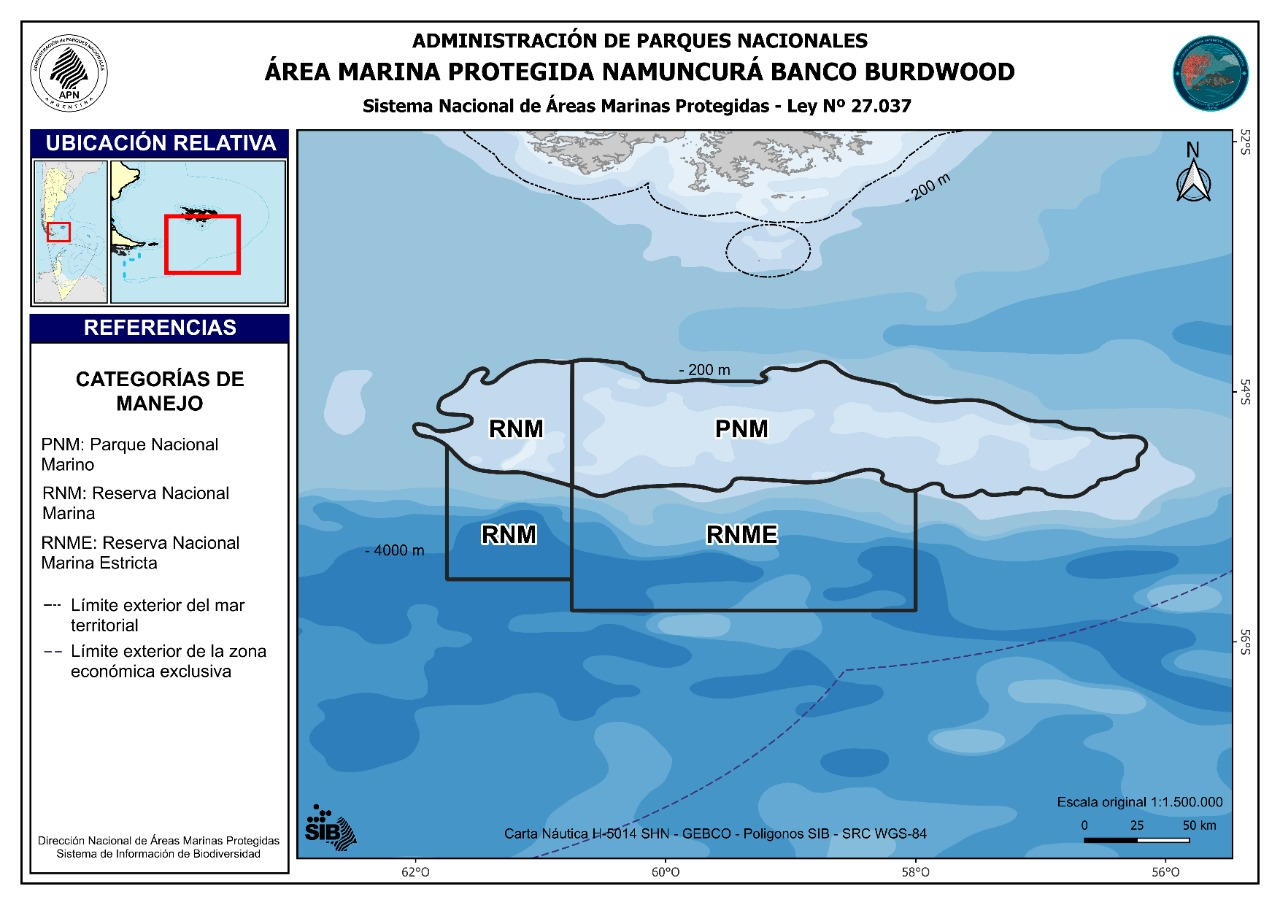
\includegraphics[width=1\linewidth]{MPABurdwood_map} \caption{Marine Protected Areas Namuncurá - Burdwood Bank I (MNR and MNP, northern section) and II (MNR and \DIFdelbeginFL \DIFdelFL{SMNR}\DIFdelendFL \DIFaddbeginFL \DIFaddFL{RMNR}\DIFaddendFL , southern section). Acronyms indicate categories according to the management plan: MNR - Marine National Reserve, MNP - Marine National Park and RMNR - Restricted Marine National Reserve.}\label{fig:figure1}
\end{figure}

\begin{figure}

{\centering \DIFdelbeginFL %DIFDELCMD < 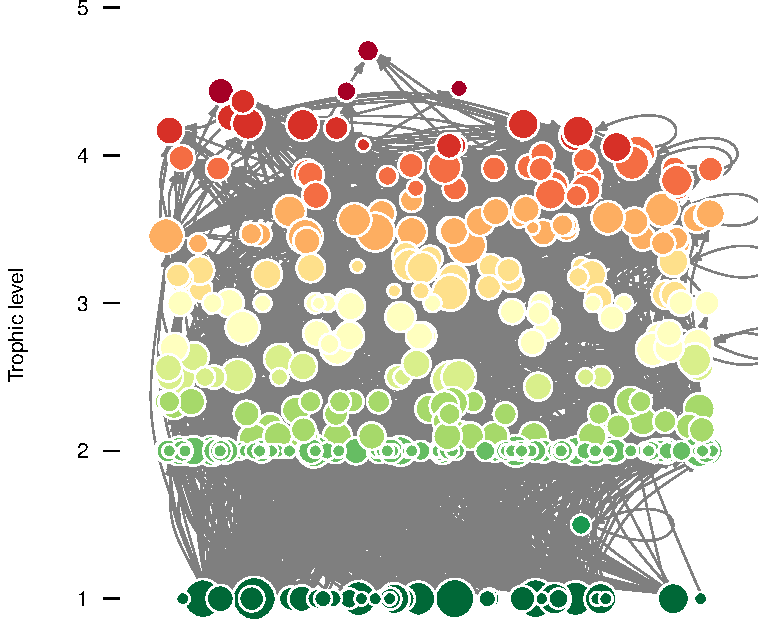
\includegraphics{OriginallySubmittedVersion_files/figure-latex/figure2-1} 
%DIFDELCMD < %%%
\DIFdelendFL \DIFaddbeginFL \includegraphics{figure2_ok} 
\DIFaddendFL 

}

\caption{Graph of the food web for the MPA Namuncurá - Burdwood Bank. Circles represent \DIFaddbeginFL \DIFaddFL{trophic }\DIFaddendFL species and arrows trophic interactions. Circle diameter is relative to the number of interactions \DIFaddbeginFL \DIFaddFL{(see legend)}\DIFaddendFL . Colour gradient indicates the trophic level.}\label{fig:figure2}
\end{figure}

\begin{figure}

{\centering \DIFdelbeginFL %DIFDELCMD < \includegraphics{OriginallySubmittedVersion_files/figure-latex/figure3-1} 
%DIFDELCMD < %%%
\DIFdelendFL \DIFaddbeginFL \includegraphics{RevisedVersion_files/figure-latex/figure3-1} 
\DIFaddendFL 

}

\caption{Degree distributions for the (A) food web, for (B) prey among predators, (C) predators among prey, and (D) for each functional group. Groups are vertically ordered by increasing trophic level (following coloration of figure 2); groups with less than 3 species were not plotted (e.g., pelagic fish). All functional groups and the species that comprise them are shown in Supplementary Material (Table S3).}\label{fig:figure3}
\end{figure}

\DIFdelbegin %DIFDELCMD < \begin{figure}
%DIFDELCMD < %%%
\DIFdelendFL \DIFaddbeginFL \newpage
\DIFaddendFL 

\DIFdelbeginFL %DIFDELCMD < {%%%
\DIFdelendFL \DIFaddbeginFL \DIFaddFL{\textbackslash begin\{figure\}
}

\DIFaddFL{\{}\DIFaddendFL \centering \DIFdelbeginFL %DIFDELCMD < \includegraphics{OriginallySubmittedVersion_files/figure-latex/figure4-1} 
%DIFDELCMD < %%%
\DIFdelendFL \DIFaddbeginFL \includegraphics{RevisedVersion_files/figure-latex/figure4-1}
\DIFaddendFL 

\DIFdelbeginFL %DIFDELCMD < }
%DIFDELCMD < %%%
\DIFdelendFL \DIFaddbeginFL \DIFaddFL{\}
}\DIFaddendFL 

\DIFdelbeginFL %DIFDELCMD < \caption{%
{%DIFAUXCMD
\DIFdelFL{Species-level properties by trophic level: (A) trophic similarity, (B) closeness, (C) betweenness, and (D) topological role. Each point represents a species. Linear regressions for betweenness ($y = 74.97x - 117.35, R^2 = 0.05, p-value < 0.01$), closeness ($y = 9.33e-06x - 9.31e-4, R^2 = 0.003, p-value = 0.15$) and trophic similarity ($y = -0.02x + 0.11 , R^2 = 0.07, p-value < 0.01$). Note that for panels A, B and C only species with TLs equal or greater than 2 were considered.}}%DIFAUXCMD
\DIFdelendFL \DIFaddbeginFL \DIFaddFL{\textbackslash caption\{Species-level properties by trophic level: (A)
betweenness, (B) closeness, (C) trophic similarity, and (D) topological
role. Each point represents a species. Note that for panels A, B and C
only species with TLs equal or greater than 2 were considered. In the
boxplot (D), the horizontal line in the middle of each box represents
the median of the data, the colored box represents the interquartile
range (range between the 1st, or 25th percentile, and 3rd, or 75th
percentile, quartile), containing the middle 50\% of data
points.\}}\DIFaddendFL \label{fig:figure4} \DIFdelbeginFL %DIFDELCMD < \end{figure}
%DIFDELCMD < %%%
\DIFdelend \DIFaddbegin \DIFadd{\textbackslash end\{figure\}
}\DIFaddend 

\newpage

\subsection*{References}\label{references}
\addcontentsline{toc}{subsection}{References}

\phantomsection\label{refs}
\begin{CSLReferences}{1}{0}
\bibitem[\citeproctext]{ref-Acha2004}
Acha, E.M., Mianzan, H.W., Guerrero, R.A., Favero, M., Bava, J., 2004.
\href{https://doi.org/10.1016/j.jmarsys.2003.09.005}{Marine fronts at
the continental shelves of austral {South America}: {Physical} and
ecological processes}. Journal of Marine Systems 44, 83--105.

\bibitem[\citeproctext]{ref-AdministraciondeParquesNacionales2022}
Administración de Parques Nacionales, 2022. {Plan de gesti{ó}n AMP
Namuncur{á} Banco Burdwood}.

\bibitem[\citeproctext]{ref-Albert2002}
Albert, R., Barabási, A.-L., 2002.
\href{https://doi.org/10.1103/RevModPhys.74.47}{Statistical mechanics of
complex networks}. Reviews of Modern Physics 74, 47--97.

\bibitem[\citeproctext]{ref-Albert2000}
Albert, R., Jeong, H., Barabási, A.-L., 2000.
\href{https://doi.org/10.1038/35019019}{Error and attack tolerance of
complex networks}. Nature 406, 378--382.

\bibitem[\citeproctext]{ref-Arkhipkin2013}
Arkhipkin, A., Laptikhovsky, V., 2013.
\href{https://doi.org/10.1111/jfb.12217}{From gelatinous to muscle food
chain: Rock cod {Patagonotothen} ramsayi recycles coelenterate and
tunicate resources on the {Patagonian Shelf}}. Journal of Fish Biology
83, 1210--1220.

\bibitem[\citeproctext]{ref-Bascompte2009}
Bascompte, J., 2009.
\href{https://doi.org/10.1126/science.1170749}{Disentangling the {Web}
of {Life}}. Science 325, 416--419.

\DIFaddbegin \bibitem[\citeproctext]{ref-Bax2022}
\DIFadd{Bax, N., Barnes, D.K.A., Pineda-Metz, S.E.A., Pearman, T., Diesing, M.,
Carter, S., Downey, R.V., Evans, C.D., Brickle, P., Baylis, A.M.M.,
Adler, A.M., Guest, A., Layton, K.K.S., Brewin, P.E., Bayley, D.T.I.,
2022. Towards }{\DIFadd{Incorporation}} \DIFadd{of }{\DIFadd{Blue Carbon}} \DIFadd{in }{\DIFadd{Falkland Islands
Marine Spatial Planning}}\DIFadd{: }{\DIFadd{A Multi-Tiered Approach}}\DIFadd{. Frontiers in Marine
Science 9.
}

\DIFaddend \bibitem[\citeproctext]{ref-Belleggia2008a}
Belleggia, M., Mabragaña, E., Figueroa, D.E., Scenna, L.B., Barbini,
S.A., Astarloa, J.M.D. de, 2008.
\href{https://doi.org/10.3989/scimar.2008.72n4701}{Food habits of the
broad nose skate, {\emph{Bathyraja}}{ \emph{Brachyurops}}
({Chondrichthyes}, {Rajidae}), in the south-west {Atlantic}}. Scientia
Marina 72, 701--710.

\bibitem[\citeproctext]{ref-Bellegia2014}
Bellegia, M., Scenna, L., Barbini, S.A., Figueroa, D.E., Díaz de
Astarloa, J.M., 2014.
\href{https://doi.org/10.26028/CYBIUM/2014-384-012}{The diets of four
{Bathyraja} skates ({Elasmobranchii}, {Arhynchobatidae}) from the
{Southwest Atlantic}}.

\DIFaddbegin \bibitem[\citeproctext]{ref-Bergagna2020}
\DIFadd{Bergagna, L., Chiesa, I., Álvarez, Y.P., Ceballos, S.G., Boy, C.C.,
Riccialdelli, L., Lovrich, G.A., 2020. }{\DIFadd{En el fondo el Banco es bueno}}\DIFadd{.
La Lupa. Colecci}{\DIFadd{ó}}\DIFadd{n Fueguina de Divulgaci}{\DIFadd{ó}}\DIFadd{n Cient}{\DIFadd{í}}\DIFadd{fica 20--24.
}

\bibitem[\citeproctext]{ref-Bergagnainrev}
\DIFadd{Bergagna, L., Riccialdelli, L., Lovrich, G.A., in rev. Blue carbon in
benthic community in the }{\DIFadd{Burdwood Bank}}\DIFadd{.
}

\DIFaddend \bibitem[\citeproctext]{ref-Bertola2018}
Bértola, G., Olguín Salinas, H., Alder, V.A., 2018. Distribuci{ó}n
espacial de {Rhizosolenia} crassa, {\textquestiondown}especie clave del
banco burdwood? In: Libro de Res{ú}menes {X Jornadas Nacionales} de
{Ciencias} Del {Mar}. {Ciudad Aut{ó}noma de Buenos Aires, Argentina}.

\bibitem[\citeproctext]{ref-Bornatowski2017}
Bornatowski, H., Barreto, R., Navia, A.F., de Amorim, A.F., 2017.
\href{https://doi.org/10.1111/maec.12407}{Topological redundancy and
{``small-world''} patterns in a food web in a subtropical ecosystem of
{Brazil}}. Marine Ecology 38, e12407.

\bibitem[\citeproctext]{ref-Borrvall2000}
Borrvall, C., Ebenman, B., Tomas Jonsson, T.J., 2000.
\href{https://doi.org/10.1046/j.1461-0248.2000.00130.x}{Biodiversity
lessens the risk of cascading extinction in model food webs}. Ecology
Letters 3, 131--136.

\bibitem[\citeproctext]{ref-Brose2019}
Brose, U., Archambault, P., Barnes, A.D., Bersier, L.-F., Boy, T.,
Canning-Clode, J., Conti, E., Dias, M., Digel, C., Dissanayake, A.,
Flores, A.A.V., Fussmann, K., Gauzens, B., Gray, C., Häussler, J., Hirt,
M.R., Jacob, U., Jochum, M., Kéfi, S., McLaughlin, O., MacPherson, M.M.,
Latz, E., Layer-Dobra, K., Legagneux, P., Li, Y., Madeira, C., Martinez,
N.D., Mendonça, V., Mulder, C., Navarrete, S.A., O'Gorman, E.J., Ott,
D., Paula, J., Perkins, D., Piechnik, D., Pokrovsky, I., Raffaelli, D.,
Rall, B.C., Rosenbaum, B., Ryser, R., Silva, A., Sohlström, E.H.,
Sokolova, N., Thompson, M.S.A., Thompson, R.M., Vermandele, F., Vinagre,
C., Wang, S., Wefer, J.M., Williams, R.J., Wieters, E., Woodward, G.,
Iles, A.C., 2019.
\href{https://doi.org/10.1038/s41559-019-0899-x}{Predator traits
determine food-web architecture across ecosystems}. Nature Ecology \&
Evolution 3, 919--927.

\bibitem[\citeproctext]{ref-Bruno2023a}
Bruno, D.O., Valencia-Carrasco, C., Paci, M.A., Leonarduzzi, E., Castro,
L., Riccialdelli, L., Iachetti, C.M., Cadaillon, A., Giesecke, R.,
Schloss, I.R., Berghoff, C.F., Martín, J., Diez, M., Cabreira, A.,
Presta, M.L., Capitanio, F.L., Boy, C.C., 2023.
\href{https://doi.org/10.1016/j.jmarsys.2023.103876}{Spring plankton
energy content by size classes in two contrasting environments of a high
latitude ecosystem: {The Beagle Channel}}. Journal of Marine Systems
240, 103876.

\bibitem[\citeproctext]{ref-Catry2004}
Catry, P., Phillips, R.A., Phalan, B., Silk, J.R.D., Croxall, J.P.,
2004. \href{https://doi.org/10.3354/meps280261}{Foraging strategies of
grey-headed albatrosses {Thalassarche} chrysostoma: Integration of
movements, activity and feeding events}. Marine Ecology Progress Series
280, 261--273.

\bibitem[\citeproctext]{ref-Cirtwill2018}
Cirtwill, A.R., Dalla Riva, G.V., Gaiarsa, M.P., Bimler, M.D., Cagua,
E.F., Coux, C., Dehling, D.M., 2018.
\href{https://doi.org/10.1016/j.fooweb.2018.e00093}{A review of species
role concepts in food webs}. Food Webs 16, e00093.

\DIFaddbegin \bibitem[\citeproctext]{ref-Cleveland1992}
\DIFadd{Cleveland, W.S., Grosse, E., Shyu, W.M., 1992. Local }{\DIFadd{Regression
Models}}\DIFadd{. In: Statistical }{\DIFadd{Models}} \DIFadd{in }{\DIFadd{S}}\DIFadd{. }{\DIFadd{Wadsworth and Brooks/Cole}}\DIFadd{,
p. 68.
}

\DIFaddend \bibitem[\citeproctext]{ref-CommissionfortheConservationofAntarcticMarineLivingResourcesCCAMLR2009}
Commission for the Conservation of Antarctic Marine Living Resources
(CCAMLR), 2009. Vulnerable {Marine Ecosystem} taxa identification guide.

\bibitem[\citeproctext]{ref-Cordone2018}
Cordone, G., Marina, T.I., Salinas, V., Doyle, S.R., Saravia, L.A.,
Momo, F.R., 2018. \href{https://doi.org/10.7717/peerj.5531}{Effects of
macroalgae loss in an {Antarctic} marine food web: Applying extinction
thresholds to food web studies}. PeerJ 6, e5531.

\bibitem[\citeproctext]{ref-Cordone2020}
Cordone, G., Salinas, V., Marina, T.I., Doyle, S.R., Pasotti, F.,
Saravia, L.A., Momo, F.R., 2020.
\href{https://doi.org/10.1016/j.fooweb.2020.e00166}{Green vs brown food
web: {Effects} of habitat type on multidimensional stability proxies for
a highly-resolved {Antarctic} food web}. Food Webs 25, e00166.

\bibitem[\citeproctext]{ref-Cossi2021}
Cossi, P.F., Ojeda, M., Chiesa, I.L., Rimondino, G.N., Fraysse, C.,
Calcagno, J., Pérez, A.F., 2021.
\href{https://doi.org/10.1007/s00300-021-02959-5}{First evidence of
microplastics in the {Marine Protected Area Namuncur{á}} at {Burdwood
Bank}, {Argentina}: A study on {Henricia} obesa and {Odontaster}
penicillatus ({Echinodermata}: {Asteroidea})}. Polar Biology 44,
2277--2287.

\bibitem[\citeproctext]{ref-CovattiAle2022}
Covatti Ale, M., Fischer, L., Deli Antoni, M., Diaz de Astarloa, J.M.,
Delpiani, G., 2022.
\href{https://doi.org/10.1007/s00300-022-03011-w}{Trophic ecology of the
yellowfin notothen, {Patagonotothen} guntheri ({Norman}, 1937) at the
{Marine Protected Area Namuncur{á}-Burdwood Bank}, {Argentina}}. Polar
Biology 45, 549--558.

\bibitem[\citeproctext]{ref-Csardi2006}
Csardi, Nepusz, 2006. The igraph software package for complex network
research.

\bibitem[\citeproctext]{ref-Cury2000}
Cury, P., Bakun, A., Crawford, R.J.M., Jarre, A., Quiñones, R.A.,
Shannon, L.J., Verheye, H.M., 2000.
\href{https://doi.org/10.1006/jmsc.2000.0712}{Small pelagics in
upwelling systems: Patterns of interaction and structural changes in
{``wasp-waist''} ecosystems}. ICES Journal of Marine Science 57,
603--618.

\DIFdelbegin \bibitem[\citeproctext]{ref-Day2013}
\DIFdel{Day, R.H., Weingartner, T.J., Hopcroft, R.R., Aerts, L.A.M., Blanchard,
A.L., Gall, A.E., Gallaway, B.J., Hannay, D.E., Holladay, B.A., Mathis,
J.T., Norcross, B.L., Questel, J.M., Wisdom, S.S., 2013.
}\href{https://doi.org/10.1016/j.csr.2013.02.002}{\DIFdel{The offshore
northeastern }%DIFDELCMD < {%%%
\DIFdel{Chukchi Sea}%DIFDELCMD < }%%%
\DIFdel{, }%DIFDELCMD < {%%%
\DIFdel{Alaska}%DIFDELCMD < }%%%
\DIFdel{: }%DIFDELCMD < {%%%
\DIFdel{A}%DIFDELCMD < } %%%
\DIFdel{complex high-latitude
ecosystem}}%DIFAUXCMD
\DIFdel{. Continental Shelf Research, Seasonal and interannual
dynamics of the northeastern }%DIFDELCMD < {%%%
\DIFdel{Chukchi Sea Ecosystem}%DIFDELCMD < } %%%
\DIFdel{67, 147--165.
}%DIFDELCMD < 

%DIFDELCMD < %%%
\DIFdelend \bibitem[\citeproctext]{ref-Dellabianca2023}
Dellabianca, N.A., Torres, M.A., Ordoñez, C., Fioramonti, N., Raya Rey,
A., 2023. \href{https://doi.org/10.1002/aqc.3935}{Marine protected areas
in the southern south-west {Atlantic}: {Insights} from marine top
predator communities}. Aquatic Conservation: Marine and Freshwater
Ecosystems 33, 472--487.

\bibitem[\citeproctext]{ref-Delpiani2020}
Delpiani, S.M., Bruno, D.O., Vazquez, D.M., Llompart, F., Delpiani,
G.E., Fernández, D.A., Rosso, J.J., Mabragaña, E., Díaz de Astarloa,
J.M., 2020. \href{https://doi.org/10.1007/s00300-020-02744-w}{Structure
and distribution of fish assemblages at {Burdwood Bank}, the first
{Sub-Antarctic Marine Protected Area} {``{Namuncur{á}}''} in {Argentina}
({Southwestern Atlantic Ocean})}. Polar Biology 43, 1783--1793.

\bibitem[\citeproctext]{ref-DiMauro2022}
Di Mauro, R., Castillo, S., Pérez, A., Iachetti, C.M., Silva, L., Tomba,
J.P., Chiesa, I.L., 2022.
\href{https://doi.org/10.1016/j.envpol.2022.119364}{Anthropogenic
microfibers are highly abundant at the {Burdwood Bank} seamount, a
protected sub-{Antarctic} environment in the {Southwestern Atlantic
Ocean}}. Environmental Pollution 306, 119364.

\DIFaddbegin \bibitem[\citeproctext]{ref-Diez2018}
\DIFadd{Diez, M.J., Cabreira, A.G., Madirolas, A., De Nascimento, J.M.,
Scioscia, G., Schiavini, A., Lovrich, G.A., 2018.
}\href{https://doi.org/10.1007/s00300-018-2394-2}{\DIFadd{Winter is cool:
Spatio-temporal patterns of the squat lobster }{\DIFadd{Munida}} \DIFadd{gregaria and the
}{\DIFadd{Fuegian}} \DIFadd{sprat }{\DIFadd{Sprattus}} \DIFadd{fuegensis in a sub-}{\DIFadd{Antarctic}} \DIFadd{estuarine
environment}}\DIFadd{. Polar Biology 41, 2591--2605.
}

\DIFaddend \bibitem[\citeproctext]{ref-Dormann2017}
Dormann, C.F., Fründ, J., Schaefer, H.M., 2017.
\href{https://doi.org/10.1146/annurev-ecolsys-110316-022928}{Identifying
{Causes} of {Patterns} in {Ecological Networks}: {Opportunities} and
{Limitations}}. Annual Review of Ecology, Evolution, and Systematics 48,
559--584.

\bibitem[\citeproctext]{ref-Dunne2002}
Dunne, Jennifer A., Williams, R.J., Martinez, N.D., 2002b.
\href{https://doi.org/10.1046/j.1461-0248.2002.00354.x}{Network
structure and biodiversity loss in food webs: Robustness increases with
connectance}. Ecology Letters 5, 558--567.

\bibitem[\citeproctext]{ref-Dunne2002a}
Dunne, Jennifer A., Williams, R.J., Martinez, N.D., 2002a.
\href{https://doi.org/10.1073/pnas.192407699}{Food-web structure and
network theory: {The} role of connectance and size}. Proceedings of the
National Academy of Sciences 99, 12917--12922.

\bibitem[\citeproctext]{ref-Dunne2002b}
Dunne, Jennifer A., Williams, R.J., Martinez, N.D., 2002c. Small
{Networks} but not {Small Worlds}: {Unique Aspects} of {Food Web
Structure}.

\bibitem[\citeproctext]{ref-Eklof2006}
Eklöf, A., Ebenman, B., 2006.
\href{https://doi.org/10.1111/j.1365-2656.2006.01041.x}{Species loss and
secondary extinctions in simple and complex model communities}. Journal
of Animal Ecology 75, 239--246.

\DIFaddbegin \bibitem[\citeproctext]{ref-Erdos1959}
\DIFadd{Erdös, P., Rényi, A., 1959. On random graphs. I. Publicationes
Mathematicae (Debrecen) 290--297.
}

\DIFaddend \bibitem[\citeproctext]{ref-Fagan1997}
Fagan, W.F., 1997. \href{https://doi.org/10.1086/286081}{Omnivory as a
{Stabilizing Feature} of {Natural Communities}}. The American Naturalist
150, 554--567.

\bibitem[\citeproctext]{ref-Falabella2017}
Falabella, V., 2017. {Á}rea {Marina Protegida Namuncur{á}-Banco
Burdwood}. {Contribuciones} para la l{í}nea de base y el plan de manejo.

\bibitem[\citeproctext]{ref-Fioramonti2022}
Fioramonti, N.E., Ribeiro Guevara, S., Becker, Y.A., Riccialdelli, L.,
2022. \href{https://doi.org/10.1016/j.marpolbul.2022.113365}{Mercury
transfer in coastal and oceanic food webs from the {Southwest Atlantic
Ocean}}. Marine Pollution Bulletin 175, 113365.

\bibitem[\citeproctext]{ref-Fischer2022}
Fischer, L., Covatti Ale, M., Deli Antoni, M., Díaz de Astarloa, J.M.,
Delpiani, G., 2022.
\href{https://doi.org/10.1007/s00300-022-03082-9}{Feeding ecology of the
longtail southern cod, {Patagonotothen} ramsayi ({Regan}, 1913)
({Notothenioidei}) in the {Marine Protected Area Namuncur{á}-Burdwood
Bank}, {Argentina}}. Polar Biology 45, 1483--1494.

\bibitem[\citeproctext]{ref-Florencia2023}
Florencia, M., Vazquez, D.M., Gabbanelli, V., Díaz de Astarloa, J.M.,
Mabragaña, E., 2023.
\href{https://doi.org/10.1007/s00300-023-03128-6}{Chondrichthyans from
the southern tip of {South America} with emphasis on the marine
protected area {Namuncur{á}-Burdwood Bank}: Exploring egg nursery
grounds}. Polar Biology.

\DIFaddbegin \bibitem[\citeproctext]{ref-Franco2020a}
\DIFadd{Franco, B.C., Combes, V., González Carman, V., 2020a. Subsurface }{\DIFadd{Ocean
Warming Hotspots}} \DIFadd{and }{\DIFadd{Potential Impacts}} \DIFadd{on }{\DIFadd{Marine Species}}\DIFadd{: }{\DIFadd{The
Southwest South Atlantic Ocean Case Study}}\DIFadd{. Frontiers in Marine Science
7.
}

\bibitem[\citeproctext]{ref-Franco2020}
\DIFadd{Franco, B.C., Defeo, O., Piola, A.R., Barreiro, M., Yang, H., Ortega,
L., Gianelli, I., Castello, J.P., Vera, C., Buratti, C., Pájaro, M.,
Pezzi, L.P., Möller, O.O., 2020b.
}\href{https://doi.org/10.1007/s10584-020-02783-6}{\DIFadd{Climate change impacts
on the atmospheric circulation, ocean, and fisheries in the southwest
}{\DIFadd{South Atlantic Ocean}}\DIFadd{: A review}}\DIFadd{. Climatic Change 162, 2359--2377.
}

\bibitem[\citeproctext]{ref-Franco2022}
\DIFadd{Franco, B.C., Ruiz-Etcheverry, L.A., Marrari, M., Piola, A.R., Matano,
R.P., 2022. }\href{https://doi.org/10.1029/2021GL096513}{\DIFadd{Climate }{\DIFadd{Change
Impacts}} \DIFadd{on the }{\DIFadd{Patagonian Shelf Break Front}}}\DIFadd{. Geophysical Research
Letters 49, e2021GL096513.
}

\bibitem[\citeproctext]{ref-Freeman1978}
\DIFadd{Freeman, L.C., 1978.
}\href{https://doi.org/10.1016/0378-8733(78)90021-7}{\DIFadd{Centrality in social
networks conceptual clarification}}\DIFadd{. Social Networks 1, 215--239.
}

\DIFaddend \bibitem[\citeproctext]{ref-Funes2022}
Funes, M., Saravia, L.A., Cordone, G., Iribarne, O.O., Galván, D.E.,
2022. \href{https://doi.org/10.1038/s41598-022-14363-y}{Network analysis
suggests changes in food web stability produced by bottom trawl fishery
in {Patagonia}}. Scientific Reports 12, 10876.

\DIFaddbegin \bibitem[\citeproctext]{ref-Galvan2022a}
\DIFadd{Galván, D.E., Bovcon, N.D., Cochia, P.D., González, R.A., Lattuca, M.E.,
Reinaldo, M.O., Rincón-Díaz, M.P., Romero, M.A., Vanella, F.A., Venerus,
L.A., Svendsen, G.M., 2022.
}\href{https://doi.org/10.1007/978-3-030-86676-1_9}{\DIFadd{Changes in the
}{\DIFadd{Specific}} \DIFadd{and }{\DIFadd{Biogeographic Composition}} \DIFadd{of }{\DIFadd{Coastal Fish Assemblages}}
\DIFadd{in }{\DIFadd{Patagonia}}\DIFadd{, }{\DIFadd{Driven}} \DIFadd{by }{\DIFadd{Climate Change}}\DIFadd{, }{\DIFadd{Fishing}}\DIFadd{, and }{\DIFadd{Invasion}}
\DIFadd{by }{\DIFadd{Alien Species}}}\DIFadd{. In: Helbling, E.W., Narvarte, M.A., González, R.A.,
Villafañe, V.E. (Eds.), Global }{\DIFadd{Change}} \DIFadd{in }{\DIFadd{Atlantic Coastal Patagonian
Ecosystems}}\DIFadd{: }{\DIFadd{A Journey Through Time}}\DIFadd{, Natural and }{\DIFadd{Social Sciences}} \DIFadd{of
}{\DIFadd{Patagonia}}\DIFadd{. }{\DIFadd{Springer International Publishing}}\DIFadd{, }{\DIFadd{Cham}}\DIFadd{, pp. 205--231.
}

\DIFaddend \bibitem[\citeproctext]{ref-GarciaAlonso2018}
García Alonso, V.A., Brown, D., Martín, J., Pájaro, M., Capitanio, F.L.,
2018. \href{https://doi.org/10.1007/s00300-018-2352-z}{Seasonal patterns
of {Patagonian} sprat {Sprattus} fuegensis early life stages in an open
sea {Sub-Antarctic Marine Protected Area}}. Polar Biology 41,
2167--2179.

\bibitem[\citeproctext]{ref-GarciaAlonso2020}
García Alonso, V.A., Brown, D.R., Pájaro, M., Capitanio, F.L., 2020.
Growing {Up Down South}: {Spatial} and {Temporal Variability} in {Early
Growth} of {Fuegian Sprat Sprattus} fuegensis {From} the {Southwest
Atlantic Ocean}. Frontiers in Marine Science 7.

\bibitem[\citeproctext]{ref-Gauzens2013}
Gauzens, B., Legendre, S., Lazzaro, X., Lacroix, G., 2013.
\href{https://doi.org/10.1111/j.1600-0706.2013.00266.x}{Food-web
aggregation, methodological and functional issues}. Oikos 122,
1606--1615.

\bibitem[\citeproctext]{ref-Giesecke2021}
Giesecke, R., Martín, J., Piñones, A., Höfer, J., Garcés-Vargas, J.,
Flores-Melo, X., Alarcón, E., Durrieu de Madron, X., Bourrin, F.,
González, H.E., 2021. General {Hydrography} of the {Beagle Channel}, a
{Subantarctic Interoceanic Passage} at the {Southern Tip} of {South
America}. Frontiers in Marine Science 8.

\bibitem[\citeproctext]{ref-Glorioso1995}
Glorioso, P.D., Flather, R.A., 1995.
\href{https://doi.org/10.1029/95JC00942}{A barotropic model of the
currents off {SE South America}}. Journal of Geophysical Research:
Oceans 100, 13427--13440.

\bibitem[\citeproctext]{ref-Godoy2018}
Godoy, O., Bartomeus, I., Rohr, R.P., Saavedra, S., 2018.
\href{https://doi.org/10.1016/j.tree.2018.01.007}{Towards the
{Integration} of {Niche} and {Network Theories}}. Trends in Ecology \&
Evolution 33, 287--300.

\bibitem[\citeproctext]{ref-Guerrero1999}
Guerrero, R.A., Baldoni, A.G., Benavides, H.R., 1999.
\href{http://10.0.64.26/handle/inidep/247}{Oceanographic conditions at
the southern end of the argentine continental slope}.

\bibitem[\citeproctext]{ref-Guimera2005}
Guimerà, R., Nunes Amaral, L.A., 2005.
\href{https://doi.org/10.1038/nature03288}{Functional cartography of
complex metabolic networks}. Nature 433, 895--900.

\bibitem[\citeproctext]{ref-Guinder2020}
Guinder, V.A., Malits, A., Ferronato, C., Krock, B., Garzón-Cardona, J.,
Martínez, A., 2020.
\href{https://doi.org/10.1371/journal.pone.0233156}{Microbial plankton
configuration in the epipelagic realm from the {Beagle Channel} to the
{Burdwood Bank}, a {Marine Protected Area} in {Sub-Antarctic} waters}.
PLOS ONE 15, e0233156.

\bibitem[\citeproctext]{ref-Heer2020}
Heer, H., Streib, L., Schäfer, R.B., Ruzika, S., 2020.
\href{https://doi.org/10.1371/journal.pone.0240940}{Maximising the
clustering coefficient of networks and the effects on habitat network
robustness}. PLOS ONE 15, e0240940.

\bibitem[\citeproctext]{ref-Hogg2016}
Hogg, O.T., Huvenne, V.A.I., Griffiths, H.J., Dorschel, B., Linse, K.,
2016. \href{https://doi.org/10.1038/srep33163}{Landscape mapping at
sub-{Antarctic South Georgia} provides a protocol for underpinning
large-scale marine protected areas}. Scientific Reports 6, 33163.

\bibitem[\citeproctext]{ref-IUCN2023}
IUCN, UNEP-WCMC, 2023. The world database on protected areas ({WDPA}).

\bibitem[\citeproctext]{ref-Kadoya2018}
Kadoya, T., Gellner, G., McCann, K.S., 2018.
\href{https://doi.org/10.1111/ele.13099}{Potential oscillators and
keystone modules in food webs}. Ecology Letters 21, 1330--1340.

\bibitem[\citeproctext]{ref-Kondoh2010}
Kondoh, M., Kato, S., Sakato, Y., 2010.
\href{https://doi.org/10.1890/09-2219.1}{Food webs are built up with
nested subwebs}. Ecology 91, 3123--3130.

\bibitem[\citeproctext]{ref-Kortsch2019}
Kortsch, S., Primicerio, R., Aschan, M., Lind, S., Dolgov, A.V.,
Planque, B., 2019. \href{https://doi.org/10.1111/ecog.03443}{Food-web
structure varies along environmental gradients in a high-latitude marine
ecosystem}. Ecography 42, 295--308.

\bibitem[\citeproctext]{ref-Kortsch2015}
Kortsch, S., Primicerio, R., Fossheim, M., Dolgov, A.V., Aschan, M.,
2015. \href{https://doi.org/10.1098/rspb.2015.1546}{Climate change
alters the structure of arctic marine food webs due to poleward shifts
of boreal generalists}. Proceedings of the Royal Society B: Biological
Sciences 282, 20151546.

\bibitem[\citeproctext]{ref-Lai2012}
Lai, S.-M., Liu, W.-C., Jordán, F., 2012.
\href{https://doi.org/10.1098/rsbl.2011.1167}{On the centrality and
uniqueness of species from the network perspective}. Biology Letters 8,
570--573.

\bibitem[\citeproctext]{ref-Laptikhovsky2013}
Laptikhovsky, V., Arkhipkin, A., Brickle, P., 2013.
\href{https://doi.org/10.1016/j.fishres.2013.05.006}{From small bycatch
to main commercial species: {Explosion} of stocks of rock cod
{Patagonotothen} ramsayi ({Regan}) in the {Southwest Atlantic}}.
Fisheries Research 147, 399--403.

\bibitem[\citeproctext]{ref-Latorre2023}
Latorre, M.P., Berghoff, C.F., Giesecke, R., Malits, A., Pizarro, G.,
Iachetti, C.M., Martin, J., Flores-Melo, X., Gil, M.N., Iriarte, J.L.,
Schloss, I.R., 2023.
\href{https://doi.org/10.1016/j.jmarsys.2023.103882}{Plankton metabolic
balance in the eastern {Beagle Channel} during spring}. Journal of
Marine Systems 240, 103882.

\bibitem[\citeproctext]{ref-Lopez-Gappa2018}
López-Gappa, J., Liuzzi, M.G., Zelaya, D.G., 2018.
\href{https://doi.org/10.1007/s00300-017-2234-9}{A new genus and species
of cheilostome bryozoan associated with hermit crabs in the subantarctic
{Southwest Atlantic}}. Polar Biology 41, 733--741.

\DIFaddbegin \bibitem[\citeproctext]{ref-Madirolas2000}
\DIFadd{Madirolas, A., Sánchez, R., Hansen, J., Colombo, G. Álvarez, Reta, R.,
2000. (Technical Report). }{\DIFadd{Instituto Nacional de Investigaci}{\DIFadd{ó}}\DIFadd{n y
Desarrollo Pesquero (INIDEP)}}\DIFadd{, }{\DIFadd{Mar del Plata, Argentina}}\DIFadd{.
}

\DIFaddend \bibitem[\citeproctext]{ref-Marina2018}
Marina, T.I., Salinas, V., Cordone, Georgina, Campana, G., Moreira, E.,
Deregibus, D., Torre, L., Sahade, R., Tatián, M., Barrera Oro, E., De
Troch, M., Doyle, S., Quartino, M.L., Saravia, L.A., Momo, F.R., 2018a.
\href{https://doi.org/10.1016/j.ecss.2017.10.015}{The {Food Web} of
{Potter Cove} ({Antarctica}): Complexity, structure and function}.
Estuarine, Coastal and Shelf Science 200, 141--151.

\bibitem[\citeproctext]{ref-Marina2018a}
Marina, T.I., Saravia, L.A., Cordone, G., Salinas, V., Doyle, S.R.,
Momo, F.R., 2018b.
\href{https://doi.org/10.1371/journal.pone.0198217}{Architecture of
marine food webs: {To} be or not be a {``small-world''}}. PLOS ONE 13,
e0198217.

\bibitem[\citeproctext]{ref-Marina2023}
Marina, T.I., Saravia, L.A., Kortsch, S., 2023.
\href{https://doi.org/10.5194/egusphere-2022-1518}{New insights into the
{Weddell Sea} ecosystem applying a quantitative network approach}.

\bibitem[\citeproctext]{ref-Martin2021}
Martin, J., Flores Melo, X., 2021. {{Á}rea Marina Protegida Namuncur{á}
Banco Burdwood: Aspectos f{í}sicos y biogeoqu{í}micos}.

\bibitem[\citeproctext]{ref-MartinSirito2019}
Martin Sirito, S., 2019. {Fauna asociada a corales (Octocorallia) e
hidroides (Hydrozoa) del {Á}rea Marina Protegida {``Namuncur{á}''}
(Banco Burdwood) y zonas profundas adyacentes} (PhD thesis). Universidad
Nacional de Mar del Plata (UNMdP), Argentina, {Argentina}.

\bibitem[\citeproctext]{ref-Martinez1991}
Martinez, N.D., 1991. \href{https://doi.org/10.2307/2937047}{Artifacts
or {Attributes}? {Effects} of {Resolution} on the {Little Rock Lake Food
Web}}. Ecological Monographs 61, 367--392.

\bibitem[\citeproctext]{ref-Martinez1993}
Martinez, N.D., 1993. \href{https://doi.org/10.2307/3544934}{Effects of
{Resolution} on {Food Web Structure}}. Oikos 66, 403--412.

\bibitem[\citeproctext]{ref-Martinez2021}
Martínez, P.A., Wöhler, O.C., Troccoli, G.H., Di Marco, E.J., 2021.
{An{á}lisis del impacto potencial provocado por el establecimiento de
las {á}reas marinas protegidas Namuncur{á}-Banco Burdwood I, II y
Yaganes en la pesquer{í}a argentina de merluza negra (Dissostichus
eleginoides)} (\{Technical report\} No. 23/2021). {Instituto Nacional de
Investigaci{ó}n y Desarrollo Pesquero (INIDEP), Argentina}.

\bibitem[\citeproctext]{ref-Martinez2015}
Martínez, P.A., Wöhler, O.G., Troccoli, G.H., 2015. {La evoluci{ó}n de
la pesquer{í}a de merluza negra (Dissostichus eleginoides) en el espacio
mar{í}timo argentino. Periodo 2003- 2014} (\{Technical report\} No.
11/15). {Instituto Nacional de Investigaci{ó}n y Desarrollo Pesquero
(INIDEP), Argentina}.

\bibitem[\citeproctext]{ref-Matano2019}
Matano, R.P., Palma, E.D., Combes, V., 2019.
\href{https://doi.org/10.1029/2019JC015001}{The {Burdwood Bank
Circulation}}. Journal of Geophysical Research: Oceans 124, 6904--6926.

\bibitem[\citeproctext]{ref-Matusevich2022}
Matusevich, 2022.
\href{https://doi.org/10.21203/rs.3.rs-2247873/v1}{Chondrichthyan fauna
from the {Marine Protected Area Namuncur{á}} at {Burdwood Bank}:
Exploring egg nursery grounds}.

\bibitem[\citeproctext]{ref-McCann1997}
McCann, K., Hastings, A., 1997.
\href{https://doi.org/10.1098/rspb.1997.0172}{Re{\textendash}evaluating
the omnivory{\textendash}stability relationship in food webs}.
Proceedings of the Royal Society of London. Series B: Biological
Sciences 264, 1249--1254.

\DIFdelbegin \bibitem[\citeproctext]{ref-Moles2015}
\DIFdel{Moles, J., Núñez-Pons, L., Taboada, S., Figuerola, B., Cristobo, J.,
Avila, C., 2015.
}\href{https://doi.org/10.1007/s00227-015-2714-9}{\DIFdel{Anti-predatory chemical
defences in }%DIFDELCMD < {%%%
\DIFdel{Antarctic}%DIFDELCMD < } %%%
\DIFdel{benthic fauna}}%DIFAUXCMD
\DIFdel{. Marine Biology 162, 1813--1821.
}%DIFDELCMD < 

%DIFDELCMD < %%%
\DIFdelend \bibitem[\citeproctext]{ref-Montoya2002}
Montoya, J.M., Solé, R.V., 2002.
\href{https://doi.org/10.1006/jtbi.2001.2460}{Small {World Patterns} in
{Food Webs}}. Journal of Theoretical Biology 214, 405--412.

\bibitem[\citeproctext]{ref-Montoya2003}
Montoya, J.M., Solé, R.V., 2003.
\href{https://doi.org/10.1034/j.1600-0706.2003.12031.x}{Topological
properties of food webs: From real data to community assembly models}.
Oikos 102, 614--622.

\bibitem[\citeproctext]{ref-Morales-Castilla2015}
Morales-Castilla, I., Matias, M.G., Gravel, D., Araújo, M.B., 2015.
\href{https://doi.org/10.1016/j.tree.2015.03.014}{Inferring biotic
interactions from proxies}. Trends in Ecology \& Evolution 30, 347--356.

\bibitem[\citeproctext]{ref-Neutel2002}
Neutel, A.-M., Heesterbeek, J.A.P., de Ruiter, P.C., 2002.
\href{https://doi.org/10.1126/science.1068326}{Stability in {Real Food
Webs}: {Weak Links} in {Long Loops}}. Science 296, 1120--1123.

\bibitem[\citeproctext]{ref-Newman2003}
Newman, M.E.J., 2003.
\href{https://doi.org/10.1137/S003614450342480}{The {Structure} and
{Function} of {Complex Networks}}. SIAM Review 45, 167--256.

\bibitem[\citeproctext]{ref-Nilsson2016}
Nilsson, K.A., McCann, K.S., 2016.
\href{https://doi.org/10.1007/s12080-015-0282-8}{Interaction strength
revisited{\textemdash}clarifying the role of energy flux for food web
stability}. Theoretical Ecology 9, 59--71.

\DIFdelbegin \bibitem[\citeproctext]{ref-Nunez-Pons2010}
\DIFdel{Núñez-Pons, L., Forestieri, R., Nieto, R.M., Varela, M., Nappo, M.,
Rodríguez, J., Jiménez, C., Castelluccio, F., Carbone, M., Ramos-Espla,
A., Gavagnin, M., Avila, C., 2010.
}\href{https://doi.org/10.1007/s00300-010-0819-7}{\DIFdel{Chemical defenses of
tunicates of the genus }%DIFDELCMD < {%%%
\DIFdel{Aplidium}%DIFDELCMD < } %%%
\DIFdel{from the }%DIFDELCMD < {%%%
\DIFdel{Weddell Sea}%DIFDELCMD < }
%DIFDELCMD < %%%
\DIFdel{(}%DIFDELCMD < {%%%
\DIFdel{Antarctica}%DIFDELCMD < }%%%
\DIFdel{)}}%DIFAUXCMD
\DIFdel{. Polar Biology 33, 1319--1329.
}%DIFDELCMD < 

%DIFDELCMD < %%%
\DIFdelend \bibitem[\citeproctext]{ref-Padovani2021}
Padovani, L.N., Álvarez, N., Farías, A., 2021. Alimentaci{ó}n de la
sardina fueguina ({Sprattus} fuegensis) en la regi{ó}n patag{ó}nica
austral durante la {É}poca reproductiva (Technical Report). {Instituto
Nacional de Investigaci{ó}n y Desarrollo Pesquero (INIDEP)}.

\bibitem[\citeproctext]{ref-Padovani2012}
Padovani, L.N., Viñas, M.D., Sánchez, F., Mianzan, H., 2012.
\href{https://doi.org/10.1016/j.seares.2011.10.007}{Amphipod-supported
food web: {Themisto} gaudichaudii, a key food resource for fishes in the
southern {Patagonian Shelf}}. Journal of Sea Research 67, 85--90.

\bibitem[\citeproctext]{ref-Pascual2005}
Pascual, M., Dunne, J.A., 2005. Ecological {Networks}: {Linking
Structure} to {Dynamics} in {Food Webs}. {Oxford University Press}.

\bibitem[\citeproctext]{ref-Pawar2012}
Pawar, S., Dell, A.I., Van M. Savage, 2012.
\href{https://doi.org/10.1038/nature11131}{Dimensionality of consumer
search space drives trophic interaction strengths}. Nature 486, 485.

\bibitem[\citeproctext]{ref-Piola2009}
Piola, A.R., Falabella, V., 2009. {El mar Patag{ó}nico}. In: {Atlas del
Mar Patag{ó}nico. Especies y Espacios}. {Wildlife Conservation Society y
Birdlife Internacional}, {Buenos Aires, Argentina}, pp. 54--75.

\bibitem[\citeproctext]{ref-Piola1989}
Piola, A.R., Gordon, A.L., 1989.
\href{https://doi.org/10.1016/0198-0149(89)90015-0}{Intermediate waters
in the southwest {South Atlantic}}. Deep Sea Research Part A.
Oceanographic Research Papers 36, 1--16.

\bibitem[\citeproctext]{ref-Poisot2014}
Poisot, T., Gravel, D., 2014.
\href{https://doi.org/10.7717/peerj.251}{When is an ecological network
complex? {Connectance} drives degree distribution and emerging network
properties}. PeerJ 2, e251.

\bibitem[\citeproctext]{ref-Pomeranz2019}
Pomeranz, J.P.F., Thompson, R.M., Poisot, T., Harding, J.S., 2019.
\href{https://doi.org/10.1111/2041-210X.13125}{Inferring
predator{\textendash}prey interactions in food webs}. Methods in Ecology
and Evolution 10, 356--367.

\bibitem[\citeproctext]{ref-Presta2023}
Presta, M.L., Riccialdelli, L., Bruno, D.O., Castro, L.R., Fioramonti,
N.E., Florentín, O.V., Berghoff, C.F., Capitanio, F.L., Lovrich, G.A.,
2023.
\href{https://doi.org/10.1016/j.jmarsys.2023.103881}{Mesozooplankton
community structure and trophic relationships in an austral
high-latitude ecosystem ({Beagle Channel}): {The} role of bottom-up and
top-down forces during springtime}. Journal of Marine Systems 240,
103881.

\DIFdelbegin \bibitem[\citeproctext]{ref-Prieto2022}
\DIFdel{Prieto, I.M., Paola, A., Pérez, M., García, M., Blustein, G., Schejter,
L., Palermo, J.A., 2022.
}\href{https://doi.org/10.1002/cbdv.202100618}{\DIFdel{Antifouling }%DIFDELCMD < {%%%
\DIFdel{Diterpenoids}%DIFDELCMD < }
%DIFDELCMD < %%%
\DIFdel{from the }%DIFDELCMD < {%%%
\DIFdel{Sponge}%DIFDELCMD < } {%%%
\emph{\DIFdel{Dendrilla}}%DIFAUXCMD
%DIFDELCMD < }{ %%%
\emph{\DIFdel{Antarctica}}%DIFAUXCMD
%DIFDELCMD < }%%%
}%DIFAUXCMD
\DIFdel{. Chemistry \&
Biodiversity 19.
}%DIFDELCMD < 

%DIFDELCMD < %%%
\DIFdelend \bibitem[\citeproctext]{ref-Reta2014}
Reta, R., 2014. Oceanograf{í}a del {Banco Burdwood}: {Estado Actual} del
{Conocimiento} y {Perspectivas}.

\bibitem[\citeproctext]{ref-Riccialdelli2020}
Riccialdelli, L., Becker, Y.A., Fioramonti, N.E., Torres, M., Bruno,
D.O., Rey, A.R., Fernández, D.A., 2020.
\href{https://doi.org/10.3354/meps13524}{Trophic structure of southern
marine ecosystems: A comparative isotopic analysis from the {Beagle
Channel} to the oceanic {Burdwood Bank} area under a wasp-waist
assumption}. Marine Ecology Progress Series 655, 1--27.

\DIFaddbegin \bibitem[\citeproctext]{ref-Riccialdelli2010}
\DIFadd{Riccialdelli, L., Newsome, S.D., Fogel, M.L., Goodall, R.N.P., 2010.
}\href{https://doi.org/10.3354/meps08826}{\DIFadd{Isotopic assessment of prey and
habitat preferences of a cetacean community in the southwestern }{\DIFadd{South
Atlantic Ocean}}}\DIFadd{. Marine Ecology Progress Series 418, 235--248.
}

\DIFaddend \bibitem[\citeproctext]{ref-Roberts2017}
Roberts, C.M., O'Leary, B.C., McCauley, D.J., Cury, P.M., Duarte, C.M.,
Lubchenco, J., Pauly, D., Sáenz-Arroyo, A., Sumaila, U.R., Wilson, R.W.,
Worm, B., Castilla, J.C., 2017.
\href{https://doi.org/10.1073/pnas.1701262114}{Marine reserves can
mitigate and promote adaptation to climate change}. Proceedings of the
National Academy of Sciences 114, 6167--6175.

\bibitem[\citeproctext]{ref-Rodriguez2022}
Rodriguez, I.D., Marina, T.I., Schloss, I.R., Saravia, L.A., 2022.
\href{https://doi.org/10.1016/j.marenvres.2022.105561}{Marine food webs
are more complex but less stable in sub-{Antarctic} ({Beagle Channel},
{Argentina}) than in {Antarctic} ({Potter Cove}, {Antarctic Peninsula})
regions}. Marine Environmental Research 174, 105561.

\DIFdelbegin \bibitem[\citeproctext]{ref-RojodeAlmeida2010}
\DIFdel{Rojo de Almeida, M.T., Siless, G.E., Perez, C.D., Veloso, M.J.,
Schejter, L., Puricelli, L., Palermo, J.A., 2010.
}\href{https://doi.org/10.1021/np100337j}{\DIFdel{Dolabellane }%DIFDELCMD < {%%%
\DIFdel{Diterpenoids}%DIFDELCMD < } %%%
\DIFdel{from
the }%DIFDELCMD < {%%%
\DIFdel{South Atlantic Gorgonian}%DIFDELCMD < } {%%%
\emph{\DIFdel{Convexella}}%DIFAUXCMD
%DIFDELCMD < }{
%DIFDELCMD < %%%
\emph{\DIFdel{Magelhaenica}}%DIFAUXCMD
%DIFDELCMD < }%%%
}%DIFAUXCMD
\DIFdel{. Journal of Natural Products 73, 1714--1717.
}%DIFDELCMD < 

%DIFDELCMD < %%%
\DIFdelend \bibitem[\citeproctext]{ref-Sala2018}
Sala, E., Lubchenco, J., Grorud-Colvert, K., Novelli, C., Roberts, C.,
Sumaila, U.R., 2018.
\href{https://doi.org/10.1016/j.marpol.2018.02.004}{Assessing real
progress towards effective ocean protection}. Marine Policy 91, 11--13.

\bibitem[\citeproctext]{ref-Santana2013}
Santana, C.N. de, Rozenfeld, A.F., Marquet, P.A., Duarte, C.M., 2013.
\href{https://doi.org/10.3354/meps10073}{Topological properties of polar
food webs}. Marine Ecology Progress Series 474, 15--26.

\bibitem[\citeproctext]{ref-Saporiti2015}
Saporiti, F., Bearhop, S., Vales, D.G., Silva, L., Zenteno, L., Tavares,
M., Crespo, E.A., Cardona, L., 2015.
\href{https://doi.org/10.3354/meps11464}{Latitudinal changes in the
structure of marine food webs in the {Southwestern Atlantic Ocean}}.
Marine Ecology Progress Series 538, 23--34.

\bibitem[\citeproctext]{ref-Saravia2022a}
Saravia, L.A., 2022. Multiweb: {Ecological} network analyses including
multiplex networks.

\bibitem[\citeproctext]{ref-Schejter2021}
Schejter, L., Albano, M., 2021.
\href{https://doi.org/10.1007/s00300-021-02936-y}{Benthic communities at
the marine protected area {Namuncur{á}}/{Burdwood} bank, {SW Atlantic
Ocean}: Detection of vulnerable marine ecosystems and contributions to
the assessment of the rezoning process}. Polar Biology 44, 2023--2037.

\bibitem[\citeproctext]{ref-Schejter2019}
Schejter, L., Bremec, C.S., 2019.
\href{https://doi.org/10.3989/scimar.04863.10A}{Stony corals
({Anthozoa}: {Scleractinia}) of {Burdwood Bank} and neighbouring areas,
{SW Atlantic Ocean}}. Scientia Marina 83, 247--260.

\bibitem[\citeproctext]{ref-Schejter2020}
Schejter, L., Genzano, G., Gaitán, E., Perez, C.D., Bremec, C.S., 2020.
\href{https://doi.org/10.1002/aqc.3265}{Benthic communities in the
{Southwest Atlantic Ocean}: {Conservation} value of animal forests at
the {Burdwood Bank} slope}. Aquatic Conservation: Marine and Freshwater
Ecosystems 30, 426--439.

\bibitem[\citeproctext]{ref-Schejter2016}
Schejter, L., Rimondino, C., Chiesa, I., Díaz de Astarloa, J.M., Doti,
B., Elías, R., Escolar, M., Genzano, G., López-Gappa, J., Tatián, M.,
Zelaya, D.G., Cristobo, J., Perez, C.D., Cordeiro, R.T., Bremec, C.S.,
2016. \href{https://doi.org/10.1007/s00300-016-1913-2}{Namuncur{á}
{Marine Protected Area}: An oceanic hot spot of benthic biodiversity at
{Burdwood Bank}, {Argentina}}. Polar Biology 39, 2373--2386.

\bibitem[\citeproctext]{ref-Scotti2010}
Scotti, M., Jordán, F., 2010.
\href{https://doi.org/10.1556/ComEc.11.2010.1.9}{Relationships between
centrality indices and trophic levels in food webs}. Community Ecology
11, 59--67.

\bibitem[\citeproctext]{ref-Secretariatoftheconventiononbiologicaldiversity2004}
Secretariat of the convention on biological diversity, 2004. Technical
advice on the establishment and management of a national system of
marine and coastal protected areas (Technical Report No. 13).

\bibitem[\citeproctext]{ref-Smith-Ramesh2017}
Smith-Ramesh, L.M., Moore, A.C., Schmitz, O.J., 2017.
\href{https://doi.org/10.1111/gcb.13460}{Global synthesis suggests that
food web connectance correlates to invasion resistance}. Global Change
Biology 23, 465--473.

\bibitem[\citeproctext]{ref-Sole2001}
Solé, R.V., Montoya, M., 2001.
\href{https://doi.org/10.1098/rspb.2001.1767}{Complexity and fragility
in ecological networks}. Proceedings of the Royal Society of London.
Series B: Biological Sciences 268, 2039--2045.

\bibitem[\citeproctext]{ref-Spinelli2020}
Spinelli, M.L., Malits, A., García Alonso, V.A., Martín, J., Capitanio,
F.L., 2020. \href{https://doi.org/10.1016/j.jmarsys.2020.103398}{Spatial
gradients of spring zooplankton assemblages at the open ocean
sub-{Antarctic Namuncur{á} Marine Protected Area}/{Burdwood Bank}, {SW
Atlantic Ocean}}. Journal of Marine Systems 210, 103398.

\bibitem[\citeproctext]{ref-Stouffer2010}
Stouffer, D.B., Bascompte, J., 2010.
\href{https://doi.org/10.1111/j.1461-0248.2009.01407.x}{Understanding
food-web persistence from local to global scales}. Ecology Letters 13,
154--161.

\bibitem[\citeproctext]{ref-Stouffer2005}
Stouffer, D.B., Camacho, J., Guimerà, R., Ng, C.A., Nunes Amaral, L.A.,
2005. \href{https://doi.org/10.1890/04-0957}{Quantitative {Patterns} in
the {Structure} of {Model} and {Empirical Food Webs}}. Ecology 86,
1301--1311.

\DIFaddbegin \bibitem[\citeproctext]{ref-RCoreTeam2023}
\DIFadd{Team, R.C., 2023. R: }{\DIFadd{A Language}} \DIFadd{and }{\DIFadd{Environment}} \DIFadd{for }{\DIFadd{Statistical
Computing}}\DIFadd{.
}

\DIFaddend \bibitem[\citeproctext]{ref-Thebault2010}
Thébault, E., Fontaine, C., 2010.
\href{https://doi.org/10.1126/science.1188321}{Stability of {Ecological
Communities} and the {Architecture} of {Mutualistic} and {Trophic
Networks}}. Science 329, 853--856.

\bibitem[\citeproctext]{ref-Tombesi2020}
Tombesi, M.L., Rabufetti, F., Lovrich, G.A., 2020.
\href{https://www.coleccionlalupa.com.ar/index.php/lalupa/article/view/79}{Las
{Á}reas marinas protegidas en la {Argentina}}. La Lupa. Colecci{ó}n
Fueguina De divulgaci{ó}n cient{í}fica 16, 2--7\DIFdelbegin \DIFdel{.
}%DIFDELCMD < 

%DIFDELCMD < \bibitem[\citeproctext]{ref-Trathan2021}
\DIFdel{Trathan, P.N., Fielding, S., Hollyman, P.R., Murphy, E.J.,
Warwick-Evans, V., Collins, M.A., 2021.
}\href{https://doi.org/10.1093/icesjms/fsab092}{\DIFdel{Enhancing the ecosystem
approach for the fishery for }%DIFDELCMD < {%%%
\DIFdel{Antarctic}%DIFDELCMD < } %%%
\DIFdel{krill within the complex,
variable, and changing ecosystem at }%DIFDELCMD < {%%%
\DIFdel{South Georgia}%DIFDELCMD < }%%%
}%DIFAUXCMD
\DIFdel{. ICES Journal of
Marine Science 78, 2065--2081}\DIFdelend .

\bibitem[\citeproctext]{ref-Troccoli2020}
Troccoli, G.H., Aguilar, E., Martínez, P.A., Belleggia, M., 2020.
\href{https://doi.org/10.1007/s00300-020-02730-2}{The diet of the
{Patagonian} toothfish {Dissostichus} eleginoides, a deep-sea top
predator off {Southwest Atlantic Ocean}}. Polar Biology 43, 1595--1604.

\bibitem[\citeproctext]{ref-Valenzuela2018}
Valenzuela, L.O., Rowntree, V.J., Sironi, M., Seger, J., 2018.
\href{https://doi.org/10.3354/meps12722}{Stable isotopes
({\(\delta\)15N}, {\(\delta\)13C}, {\(\delta\)34S}) in skin reveal
diverse food sources used by southern right whales {Eubalaena}
australis}. Marine Ecology Progress Series 603, 243--255.

\bibitem[\citeproctext]{ref-Vazquez2018}
Vazquez, D.M., Belleggia, M., Schejter, L., Mabragaña, E., 2018.
\href{https://doi.org/10.1111/jfb.13490}{Avoiding being dragged away:
Finding egg cases of {Schroederichthys} bivius ({Chondrichthyes}:
{Scyliorhinidae}) associated with benthic invertebrates}. Journal of
Fish Biology 92, 248--253.

\bibitem[\citeproctext]{ref-Watts1998}
Watts, D.J., Strogatz, S.H., 1998.
\href{https://doi.org/10.1038/30918}{Collective dynamics of
{``small-world''} networks}. Nature 393, 440--442.

\bibitem[\citeproctext]{ref-Williams2002}
Williams, R.J., Berlow, E.L., Dunne, J.A., Barabási, A.-L., Martinez,
N.D., 2002. \href{https://doi.org/10.1073/pnas.192448799}{Two degrees of
separation in complex food webs}. Proceedings of the National Academy of
Sciences 99, 12913--12916.

\bibitem[\citeproctext]{ref-Winter2023}
Winter, A., Arkhipkin, A., 2023.
\href{https://doi.org/10.3390/fishes8010024}{Opportunistic {Survey
Analyses Reveal} a {Recent Decline} of {Skate} ({Rajiformes}) {Biomass}
in {Falkland Islands Waters}}. Fishes 8, 24.

\end{CSLReferences}

\end{document}
